\newpage
\section{Omitted Details in \cref{sec:exp}}
\label{app:exp}

\subsection{Overall Evaluation Time Using \sys{} vs Other Methods on Each Benchmark}

\subsubsection{\sys{} versus DPconv}
\label{app:total-time-dpconv-individual}

\paragraph{Histograms of speedups}
\cref{fig:overall-speedup-dpconv-individual} shows histograms of the speedups of the overall query execution time using \sys{} over using DPconv for queries in each of the four benchmarks. In DSB, JOB, and Musicbrainz, most of the queries show a speedup close to 1. In JOBLarge, however, we observe a large number of significant speedups by multiple orders of magnitude, mostly due to the high optimization time of DPconv for the large query sizes in this benchmark.

\begin{figure}[H]
    \begin{subfigure}[b]{0.49\textwidth}
        \centering
        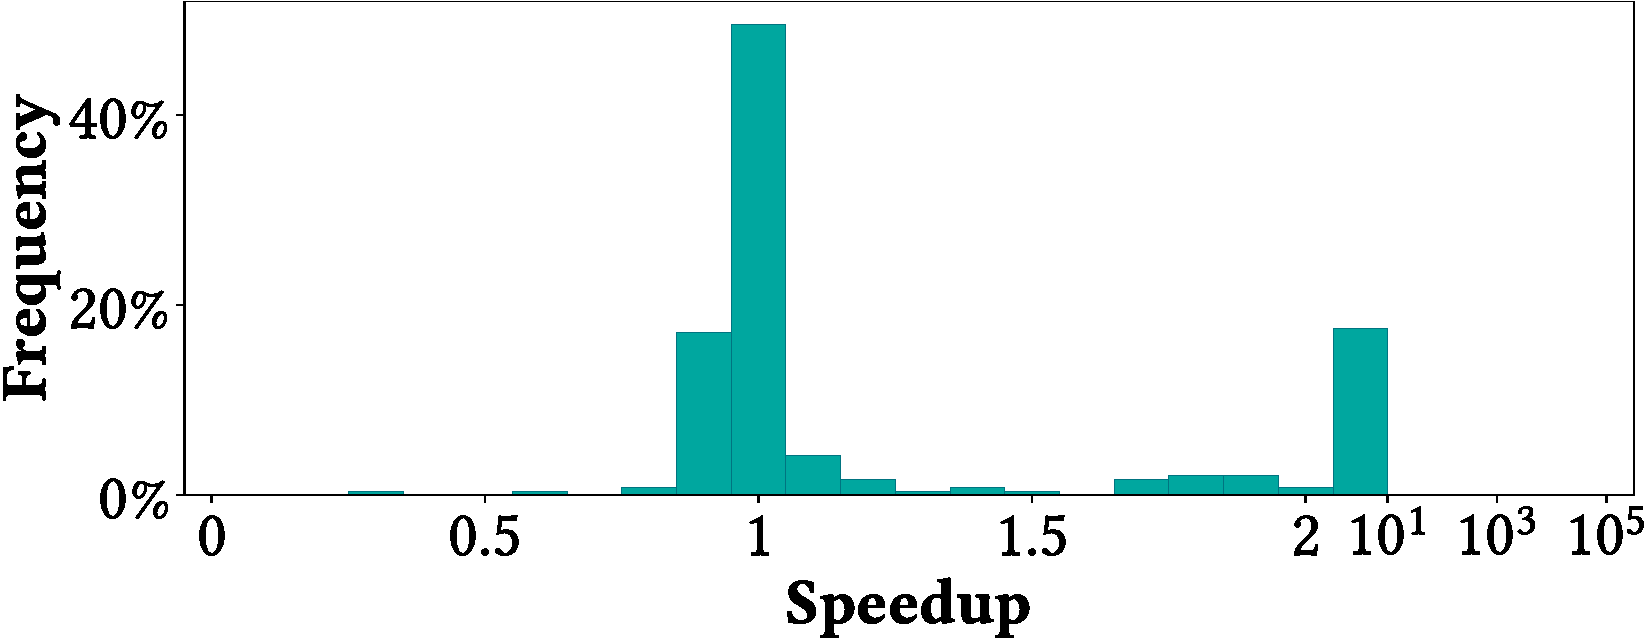
\includegraphics[width=\linewidth]{figs/exp/overall-speedups-individual/overall-speedups-over-dpconv-dsb.pdf}
        \caption{DSB}
        \label{fig:overall-speedup-dpconv-dsb}
    \end{subfigure}
    \hfill
    \begin{subfigure}[b]{0.49\textwidth}
        \centering
        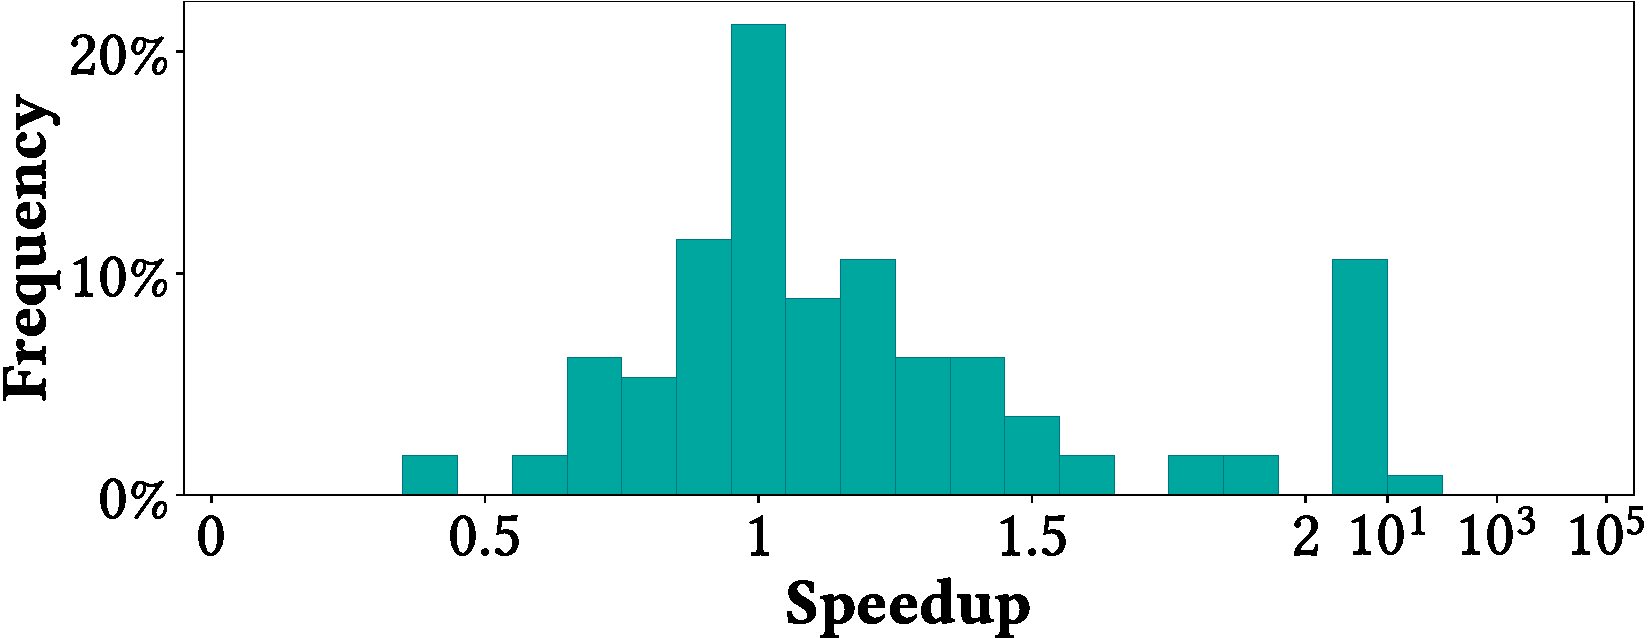
\includegraphics[width=\linewidth]{figs/exp/overall-speedups-individual/overall-speedups-over-dpconv-job-original.pdf}
        \caption{JOB}
        \label{fig:overall-speedup-dpconv-job-original}
    \end{subfigure}
    
    \vspace{0.5\baselineskip}

    \begin{subfigure}[b]{0.49\textwidth}
        \centering
        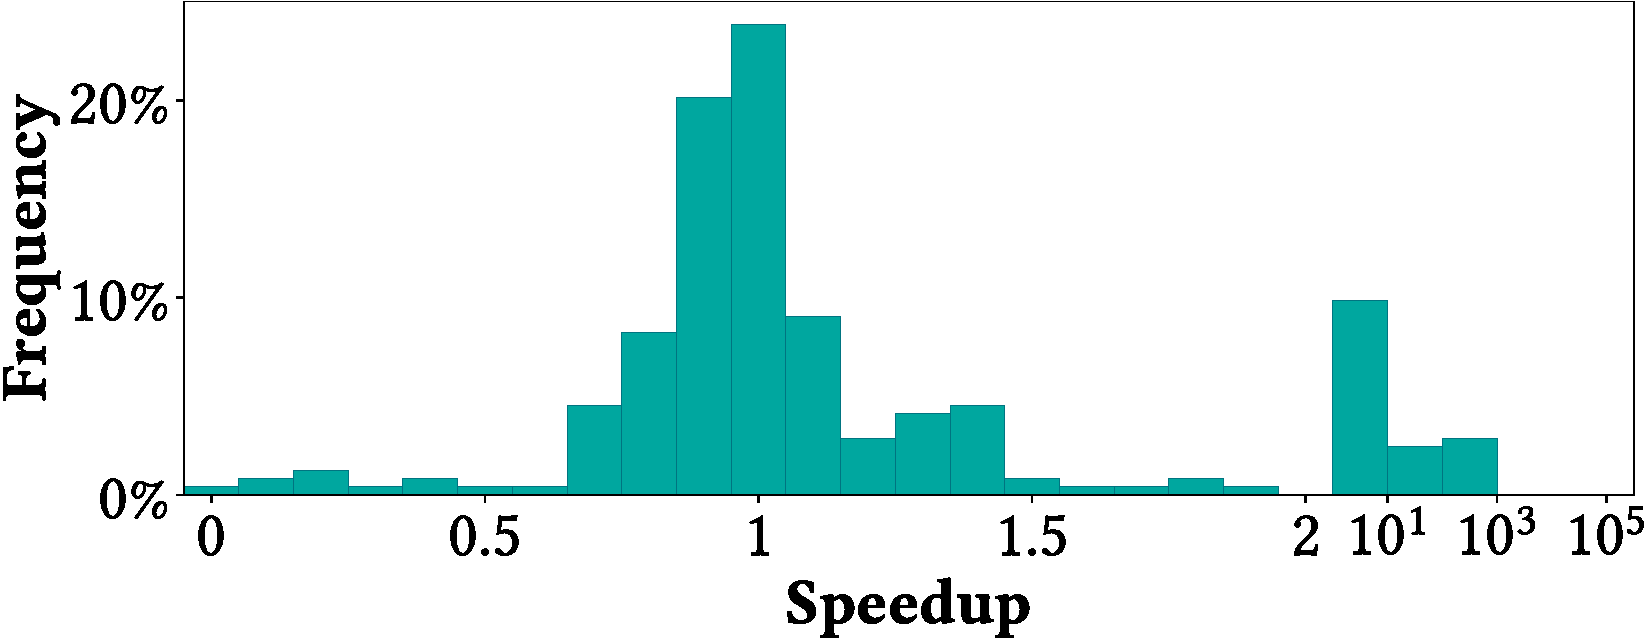
\includegraphics[width=\linewidth]{figs/exp/overall-speedups-individual/overall-speedups-over-dpconv-musicbrainz.pdf}
        \caption{Musicbrainz}
        \label{fig:overall-speedup-dpconv-musicbrainz}
    \end{subfigure}
    \hfill
    \begin{subfigure}[b]{0.49\textwidth}
        \centering
        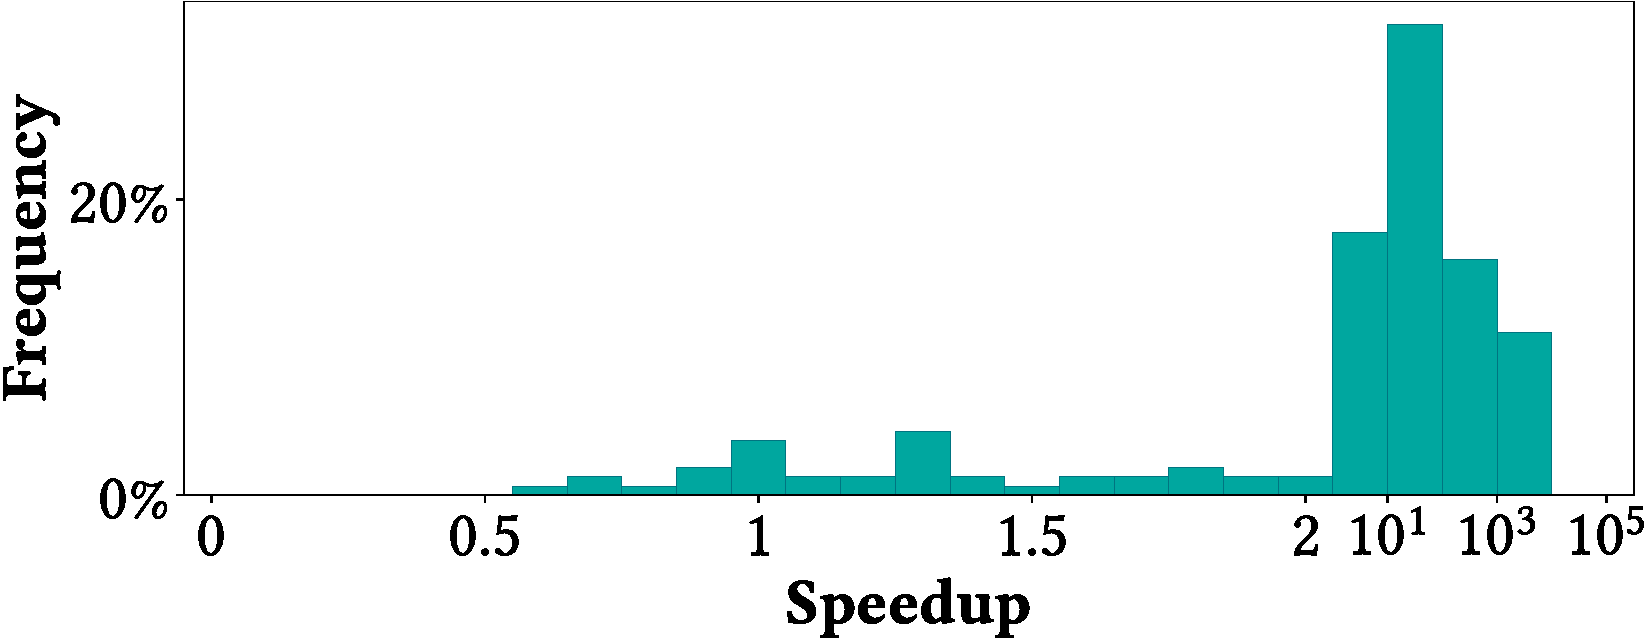
\includegraphics[width=\linewidth]{figs/exp/overall-speedups-individual/overall-speedups-over-dpconv-job-large.pdf}
        \caption{JOBLarge}
        \label{fig:overall-speedup-dpconv-job-large}
    \end{subfigure}
    \vspace{-0.5\baselineskip}
    \caption{Histograms of speedups of overall evaluation time of \sys{} over DPconv on each benchmark}
    \label{fig:overall-speedup-dpconv-individual}
\end{figure}

\paragraph{Scatter plots}
\begin{figure}
    \begin{subfigure}[b]{0.24\textwidth}
        \centering
        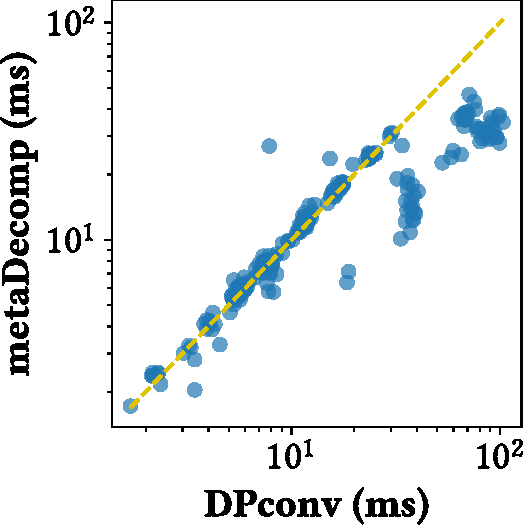
\includegraphics[width=\linewidth]{figs/exp/scatter-individual/scatter-dsb-over-dpconv.pdf}
        \vspace{-1.25\baselineskip}
        \caption{DSB}
        \label{fig:overall-scatter-dpconv-dsb}
    \end{subfigure}
    \hfill
    \begin{subfigure}[b]{0.24\textwidth}
        \centering
        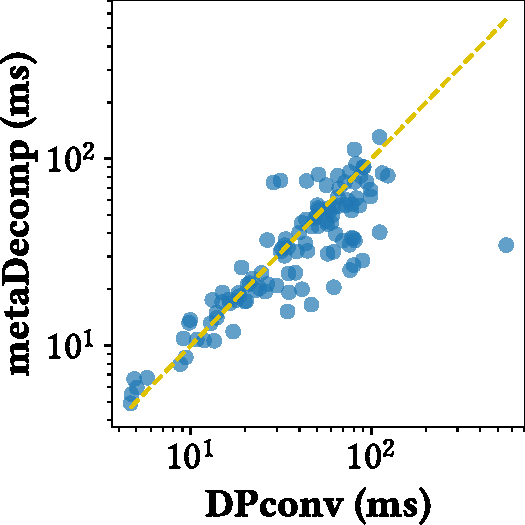
\includegraphics[width=\linewidth]{figs/exp/scatter-individual/scatter-job-original-over-dpconv.pdf}
        \vspace{-1.25\baselineskip}
        \caption{JOB}
        \label{fig:overall-scatter-dpconv-job-original}
    \end{subfigure}
    \hfill 
    \begin{subfigure}[b]{0.24\textwidth}
        \centering
        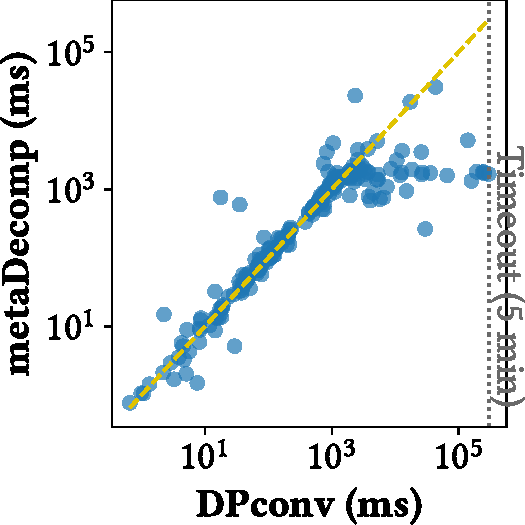
\includegraphics[width=\linewidth]{figs/exp/scatter-individual/scatter-musicbrainz-over-dpconv.pdf}
        \vspace{-1.25\baselineskip}
        \caption{Musicbrainz}
        \label{fig:overall-scatter-dpconv-musicbrainz}
    \end{subfigure}
    \hfill
    \begin{subfigure}[b]{0.24\textwidth}
        \centering
        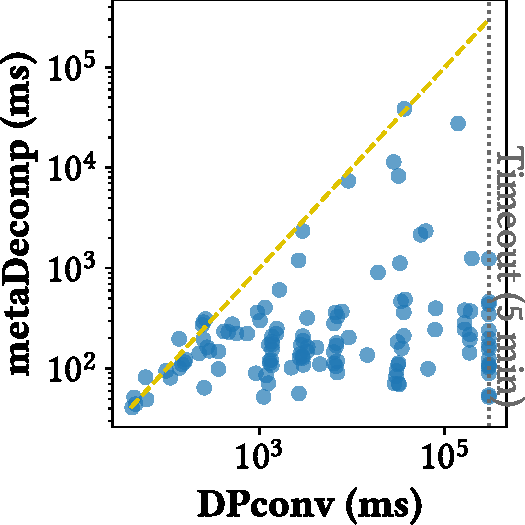
\includegraphics[width=\linewidth]{figs/exp/scatter-individual/scatter-job-large-over-dpconv.pdf}
        \vspace{-1.25\baselineskip}
        \caption{JOBLarge}
        \label{fig:overall-scatter-dpconv-job-large}
    \end{subfigure}
    \vspace{-0.5\baselineskip}
    \caption{Scatter plots of overall evaluation time of using \sys{} versus DPconv on each benchmark}
    \label{fig:overall-scatter-dpconv-individual}
\end{figure}
\cref{fig:overall-scatter-dpconv-individual} shows scatter plots of the overall evaluation time using \sys{} and DPconv, measured for queries in each of the four benchmarks. The trends that can be observed in each of the four benchmarks and the overall figure (\cref{fig:overall-scatter-dpconv}) are mostly consistent. The two approaches have similar performance for queries that takes DPconv less than 1 second ($10^3\ {\rm ms}$). For those taking DPconv more than 1 second, \sys{} starts to show significant speedups. Notably, for complex queries in Musicbrainz (\cref{fig:overall-scatter-dpconv-musicbrainz}) and JOBLarge (\cref{fig:overall-scatter-dpconv-job-large}) for which DPconv times out (taking more than 5 minutes), \sys{} can evaluate them within merely 1 second.



\newpage
\subsubsection{\sys{} versus DuckDB}
\label{app:total-time-metadecomp-duckdb-individual}

\paragraph{Histograms of speedups}
\cref{fig:overall-speedup-duckdb-individual} shows histograms of speedups of the overall evaluation time using \sys{} over DuckDB for queries in each benchmark. Most of the queries show a speedup close to 1, with some notable speedups especially for larger queries in the Musicbrainz benchmark.

\begin{figure}[H]
    \begin{subfigure}[b]{0.49\textwidth}
        \centering
        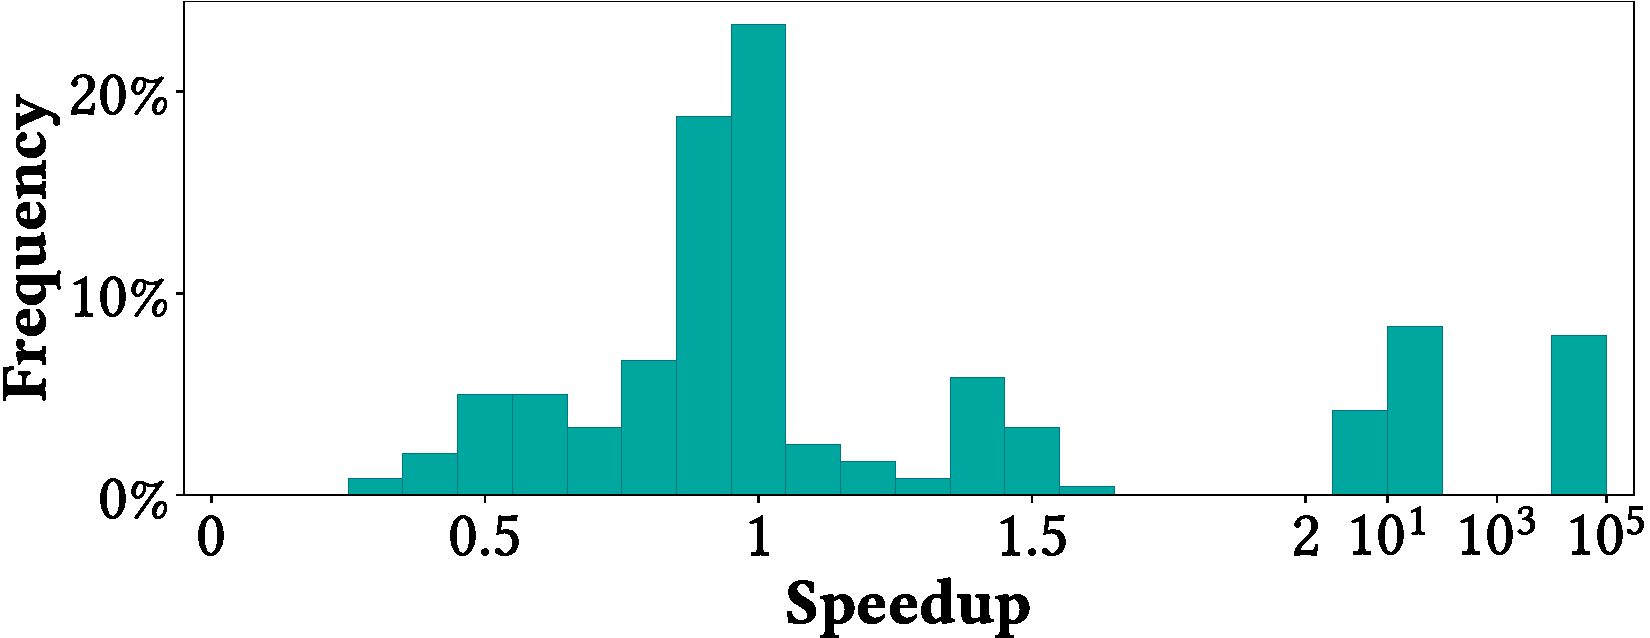
\includegraphics[width=\linewidth]{figs/exp/overall-speedups-individual/overall-speedups-over-duckdb-dsb.pdf}
        \vspace{-1.25\baselineskip}
        \caption{DSB}
        \label{fig:overall-speedup-duckdb-dsb}
    \end{subfigure}
    \hfill
    \begin{subfigure}[b]{0.49\textwidth}
        \centering
        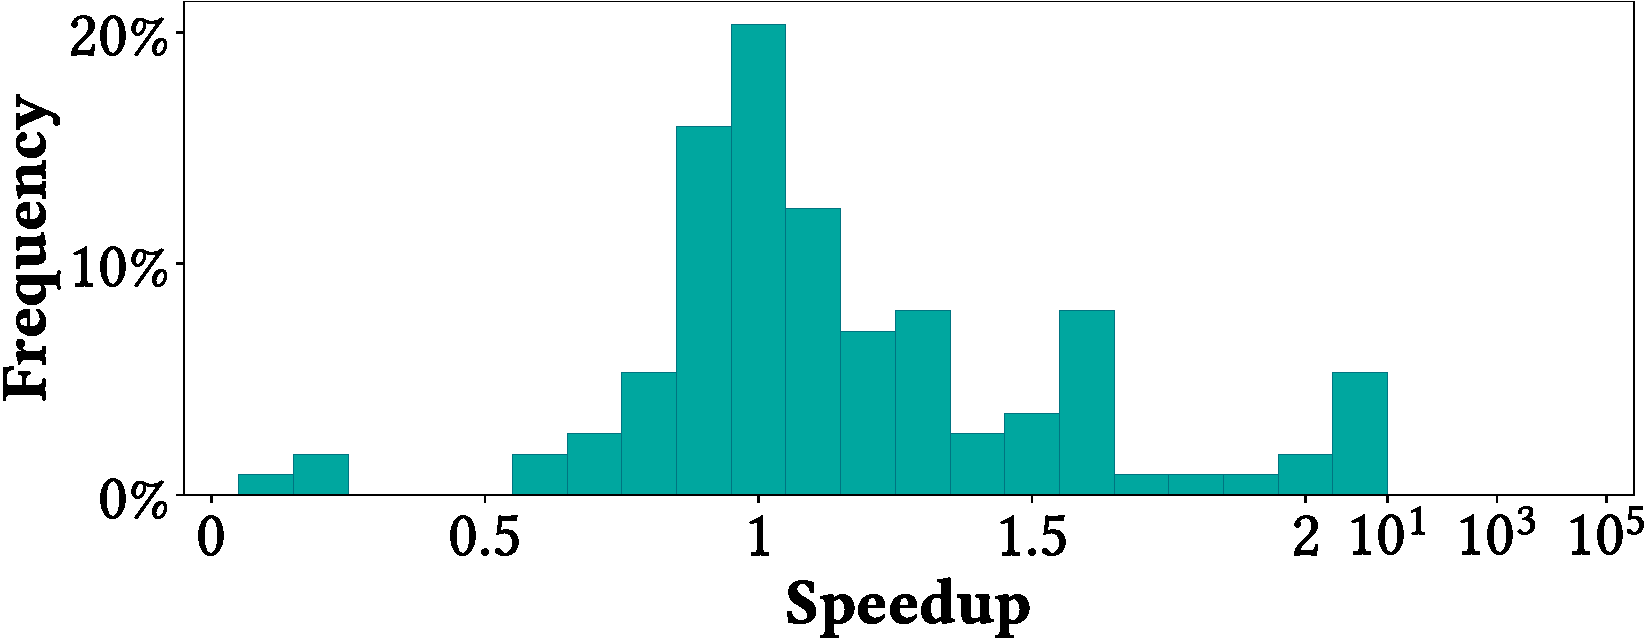
\includegraphics[width=\linewidth]{figs/exp/overall-speedups-individual/overall-speedups-over-duckdb-job-original.pdf}
        \vspace{-1.25\baselineskip}
        \caption{JOB}
        \label{fig:overall-speedup-duckdb-job-original}
    \end{subfigure}

    \vspace{0.5\baselineskip}

    \begin{subfigure}[b]{0.49\textwidth}
        \centering
        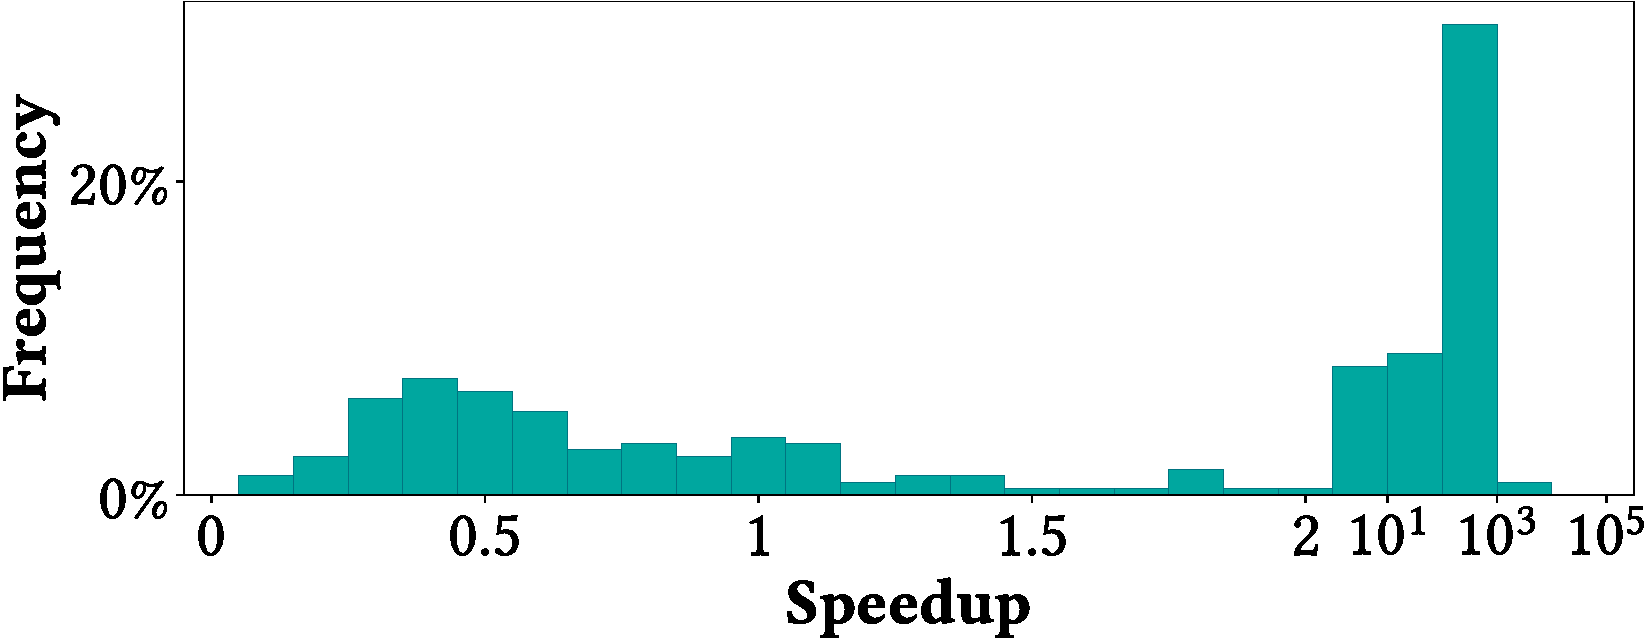
\includegraphics[width=\linewidth]{figs/exp/overall-speedups-individual/overall-speedups-over-duckdb-musicbrainz.pdf}
        \vspace{-1.25\baselineskip}
        \caption{Musicbrainz}
        \label{fig:overall-speedup-duckdb-musicbrainz}
    \end{subfigure}
    \hfill
    \begin{subfigure}[b]{0.49\textwidth}
        \centering
        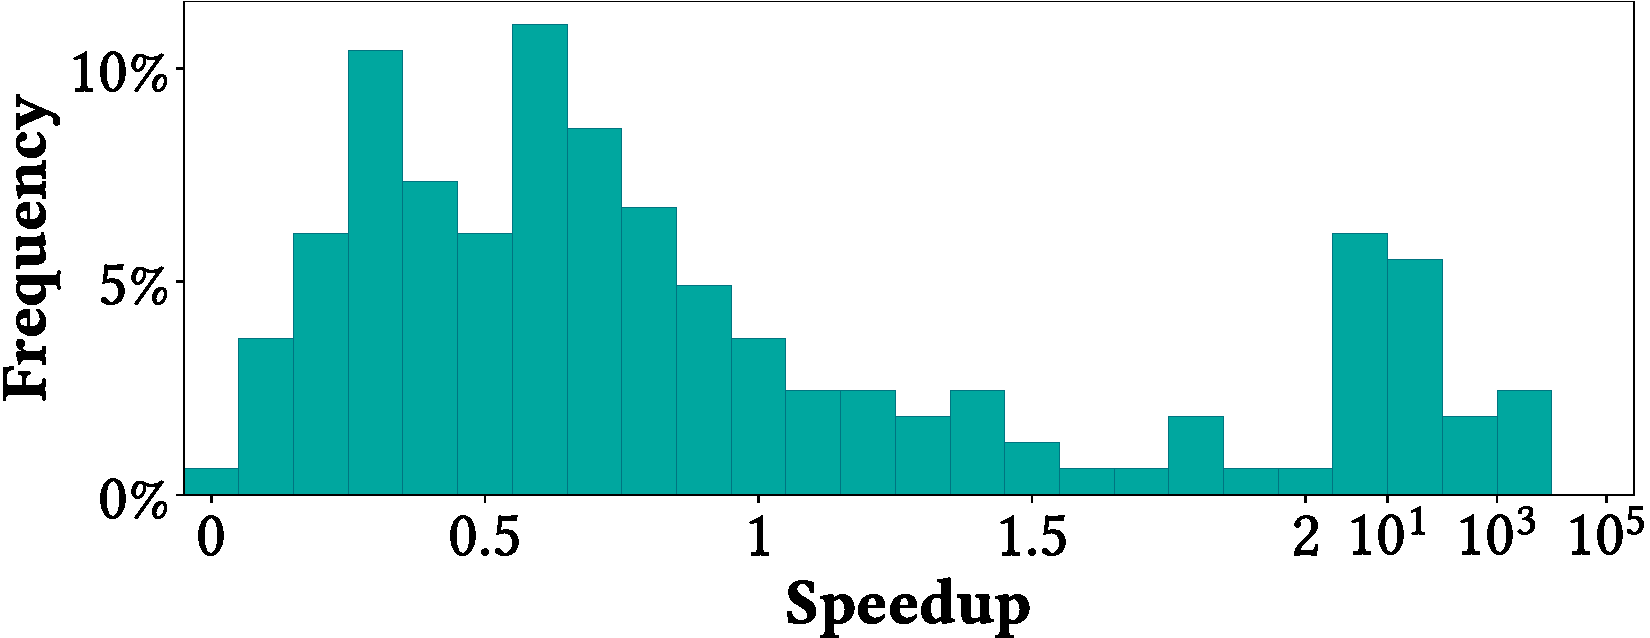
\includegraphics[width=\linewidth]{figs/exp/overall-speedups-individual/overall-speedups-over-duckdb-job-large.pdf}
        \vspace{-1.25\baselineskip}
        \caption{JOBLarge}
        \label{fig:overall-speedup-duckdb-job-large}
    \end{subfigure}
    \vspace{-0.5\baselineskip}
    \caption{Histograms of speedups of overall evaluation time of \sys{} over DuckDB on each benchmark}
    \label{fig:overall-speedup-duckdb-individual}
\end{figure}



\paragraph{Scatter plots}
\label{app:total-time-duckdb-individual}
\begin{figure}[b]
    \begin{subfigure}[b]{0.24\textwidth}
        \centering
        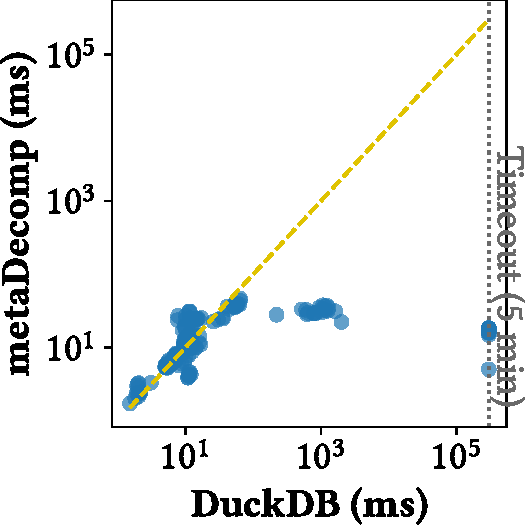
\includegraphics[width=\linewidth]{figs/exp/scatter-individual/scatter-dsb-over-duckdb.pdf}
        \vspace{-1.25\baselineskip}
        \caption{DSB}
        \label{fig:overall-scatter-duckdb-dsb}
    \end{subfigure}
    \hfill
    \begin{subfigure}[b]{0.24\textwidth}
        \centering
        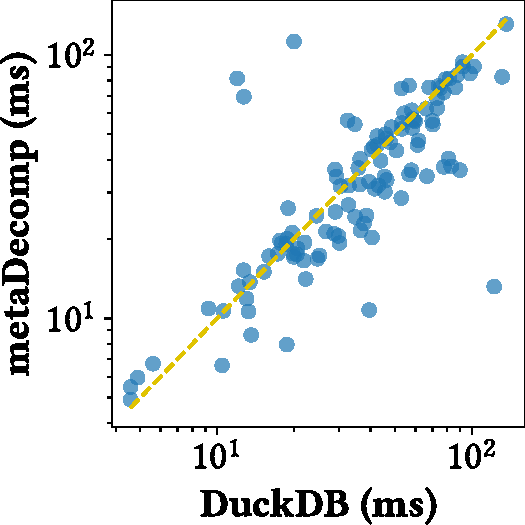
\includegraphics[width=\linewidth]{figs/exp/scatter-individual/scatter-job-original-over-duckdb.pdf}
        \vspace{-1.25\baselineskip}
        \caption{JOB}
        \label{fig:overall-scatter-duckdb-job-original}
    \end{subfigure}
    \hfill
    \begin{subfigure}[b]{0.24\textwidth}
        \centering
        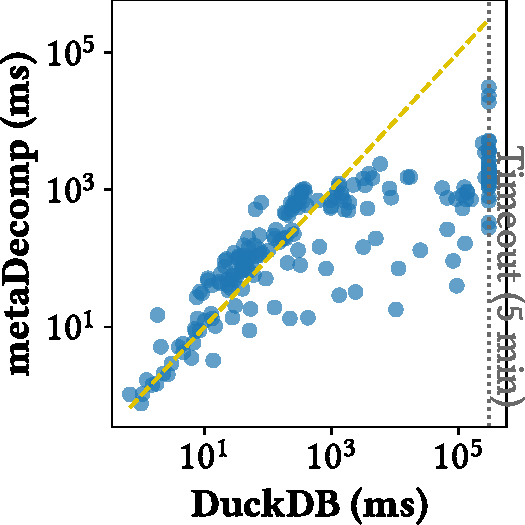
\includegraphics[width=\linewidth]{figs/exp/scatter-individual/scatter-musicbrainz-over-duckdb.pdf}
        \vspace{-1.25\baselineskip}
        \caption{Musicbrainz}
        \label{fig:overall-scatter-duckdb-musicbrainz}
    \end{subfigure}
    \hfill
    \begin{subfigure}[b]{0.24\textwidth}
        \centering
        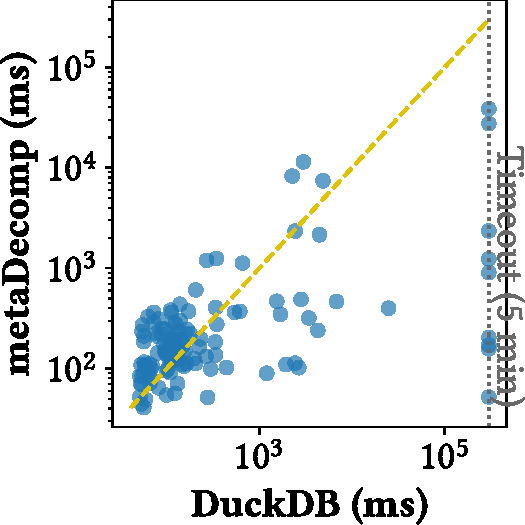
\includegraphics[width=\linewidth]{figs/exp/scatter-individual/scatter-job-large-over-duckdb.pdf}
        \vspace{-1.25\baselineskip}
        \caption{JOBLarge}
        \label{fig:overall-scatter-duckdb-job-large}
    \end{subfigure}
    \vspace{-0.5\baselineskip}
    \caption{Scatter plot of overall query evaluation time of using \sys{} versus DuckDB on each benchmark}
    \label{fig:overall-scatter-duckdb-individual}
\end{figure}
\cref{fig:overall-scatter-duckdb-individual} shows the detailed breakdown of overall query evaluation time using \sys{} and using DuckDB measured for queries in each of the four benchmarks.
With the exception of JOBLarge, all approaches have similar performance for queries that takes DuckDB less than 100 ms. For those taking DuckDB more than 100 ms, \sys{} starts to show significant speedups, mostly due to the greedy strategy of DuckDB used for large queries, which does not have optimality guarantees but may lead to highly suboptimal plans.

\subsubsection{\sys{} versus UnionDP}
\label{app:total-time-uniondp-individual}
\paragraph{Histograms of speedups}
\cref{fig:overall-speedup-uniondp-individual} shows histograms of the speedups of the overall query execution time using \sys{} over using UnionDP for queries in each of the four benchmarks. In the relatively smaller benchmarks DSB and JOB, the performance is similar. In Musicbrainz and JOBLarge, however, we observe a large number of significant speedups by multiple orders of magnitude, mostly due to the fact that UnionDP starts to use the heuristic partitioning which may lead to highly suboptimal plans.

\begin{figure}[H]
    \begin{subfigure}[b]{0.49\textwidth}
        \centering
        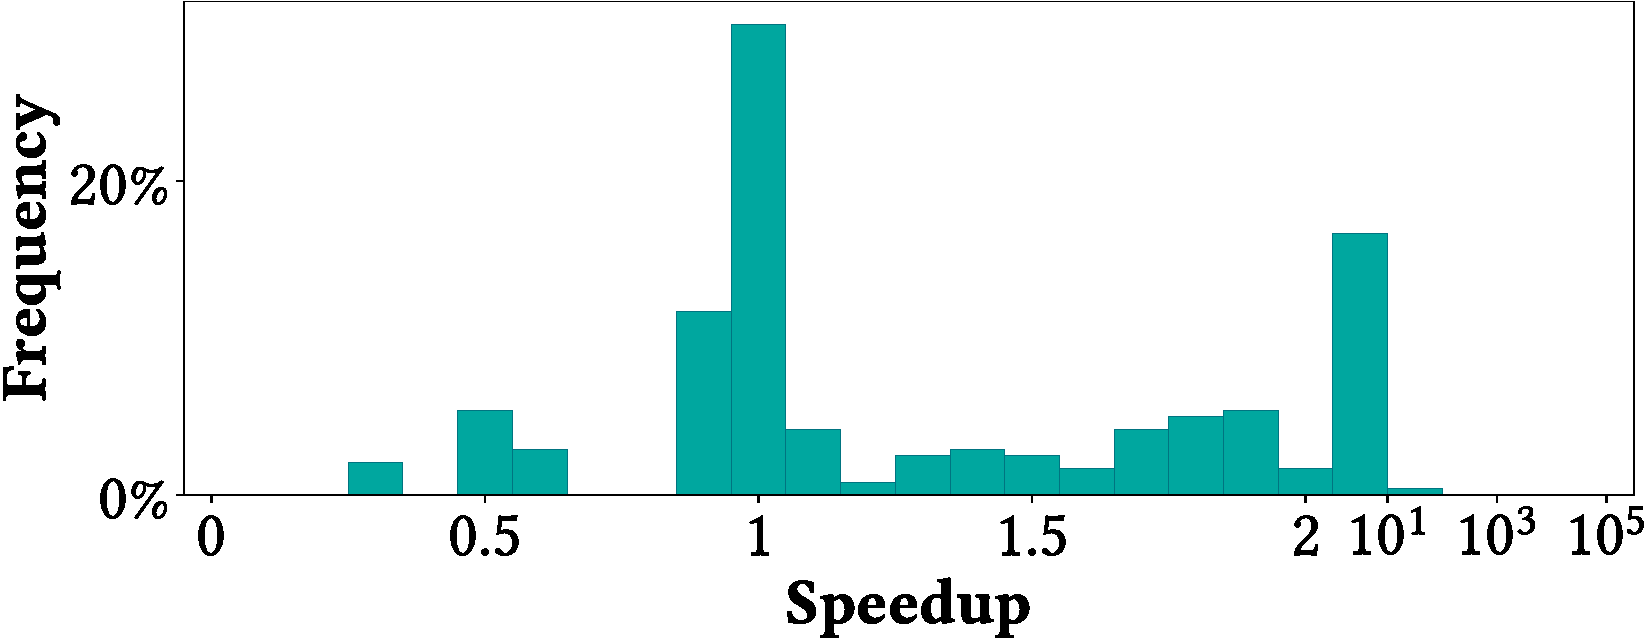
\includegraphics[width=\linewidth]{figs/exp/overall-speedups-individual/overall-speedups-over-uniondp-dsb.pdf}
        \caption{DSB}
        \label{fig:overall-speedup-uniondp-dsb}
    \end{subfigure}
    \hfill
    \begin{subfigure}[b]{0.49\textwidth}
        \centering
        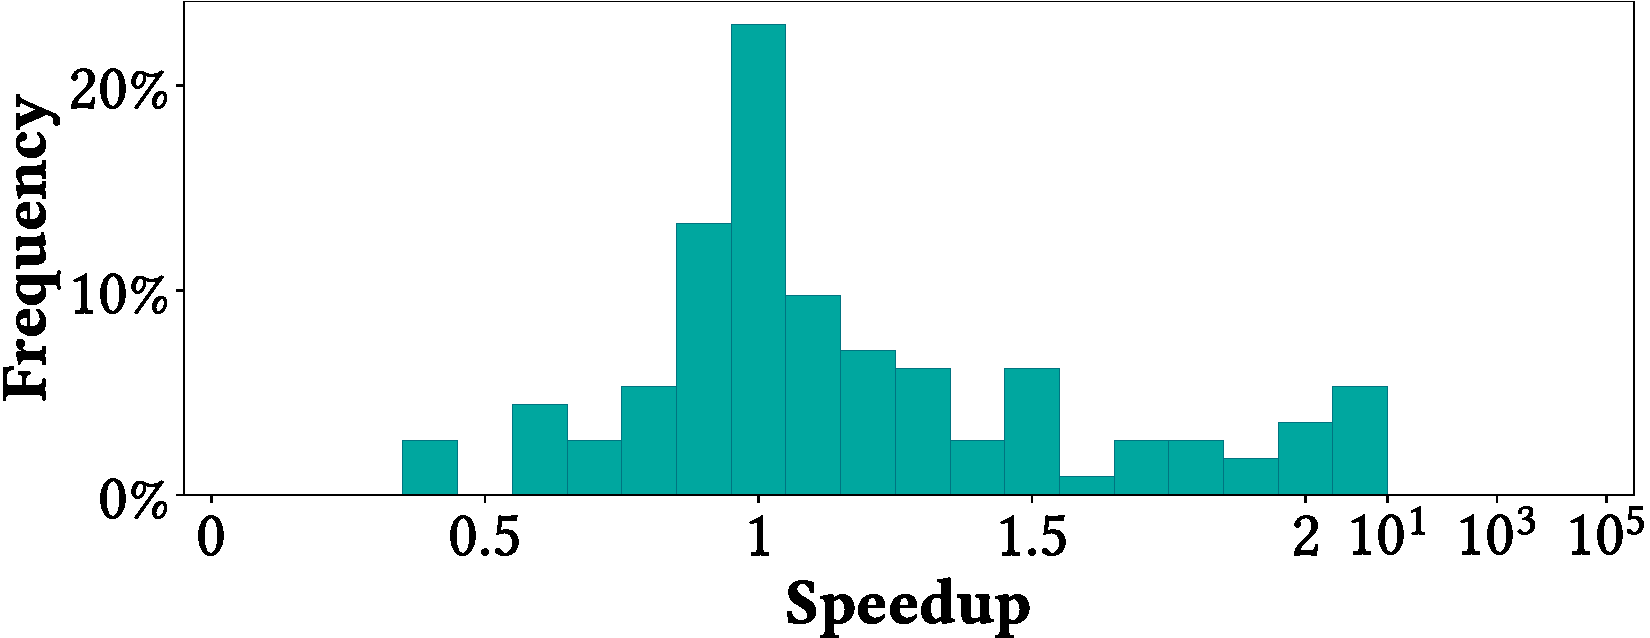
\includegraphics[width=\linewidth]{figs/exp/overall-speedups-individual/overall-speedups-over-uniondp-job-original.pdf}
        \caption{JOB}
        \label{fig:overall-speedup-uniondp-job-original}
    \end{subfigure}

    \vspace{0.5\baselineskip}

    \begin{subfigure}[b]{0.49\textwidth}
        \centering
        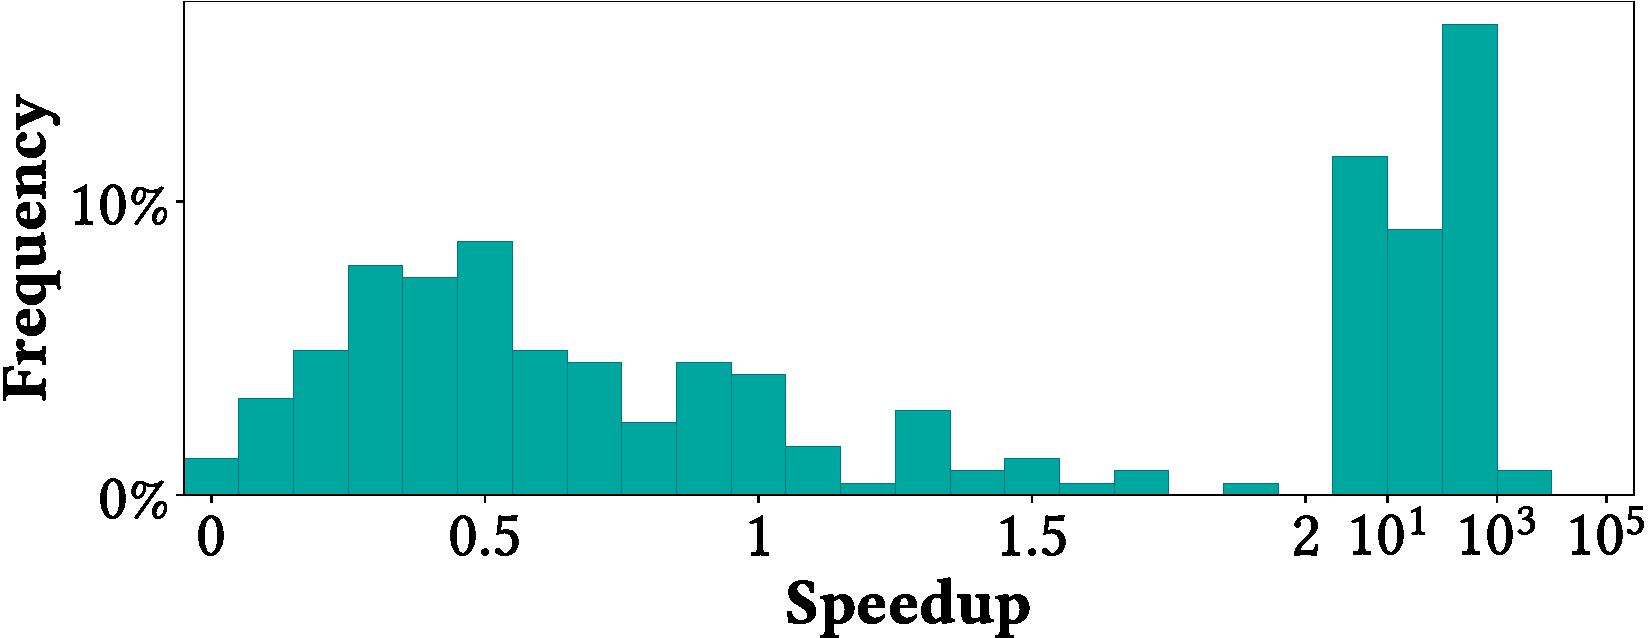
\includegraphics[width=\linewidth]{figs/exp/overall-speedups-individual/overall-speedups-over-uniondp-musicbrainz.pdf}
        \caption{Musicbrainz}
        \label{fig:overall-speedup-uniondp-musicbrainz}
    \end{subfigure}
    \hfill
    \begin{subfigure}[b]{0.49\textwidth}
        \centering
        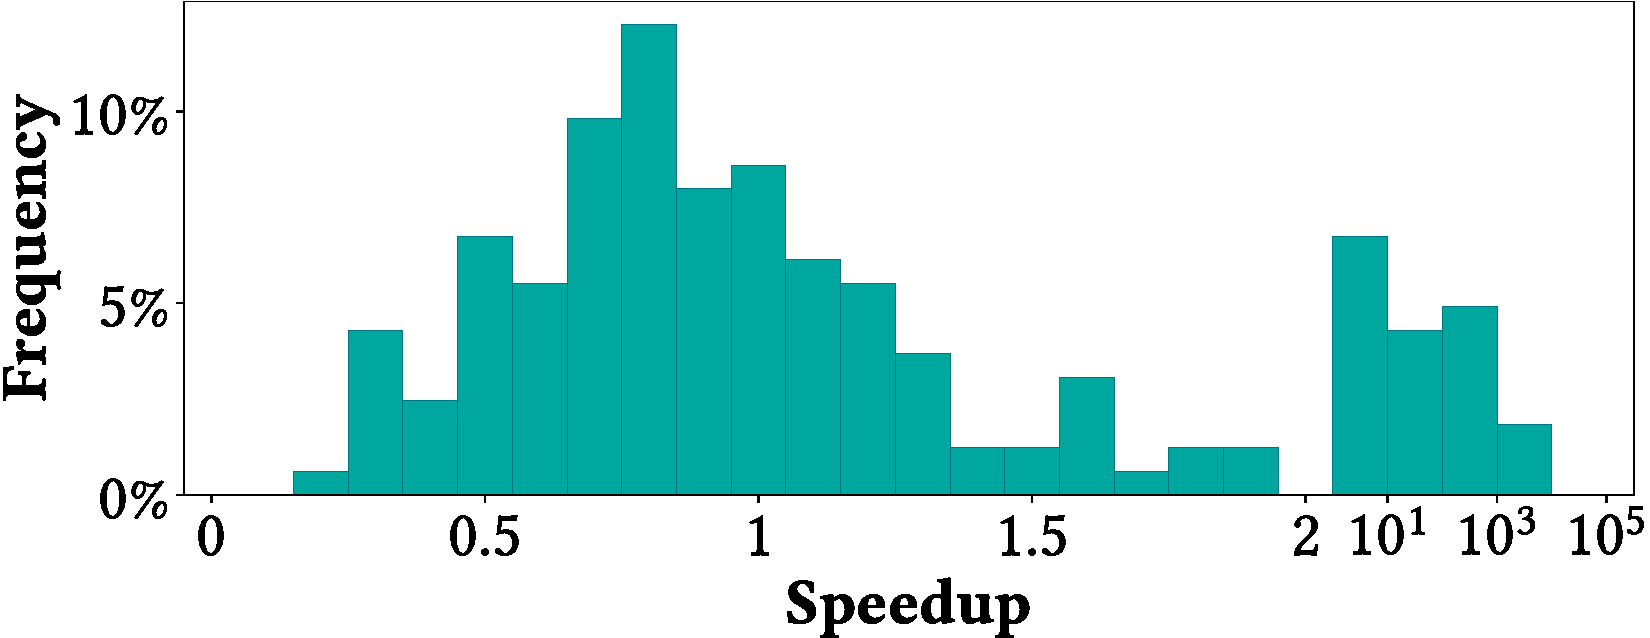
\includegraphics[width=\linewidth]{figs/exp/overall-speedups-individual/overall-speedups-over-uniondp-job-large.pdf}
        \caption{JOBLarge}
        \label{fig:overall-speedup-uniondp-job-large}
    \end{subfigure}
    \vspace{-0.5\baselineskip}
    \caption{Histograms of speedups of overall evaluation time of \sys{} over UnionDP on each benchmark}
    \label{fig:overall-speedup-uniondp-individual}
\end{figure}

\paragraph{Scatter plots} \cref{fig:overall-scatter-uniondp-individual} shows scatter plots of the overall query evaluation time using \sys{} and using UnionDP measured for queries in each of the four benchmarks. The two approaches have similar performance for queries that takes UnionDP less than 1 second ($10^3\ {\rm ms}$). For those taking UnionDP more than 1 second, \sys{} starts to show significant speedups. This is especially the case in the Musicbrainz and JOBLarge benchmarks.

\begin{figure}[H]
    \begin{subfigure}[b]{0.24\textwidth}
        \centering
        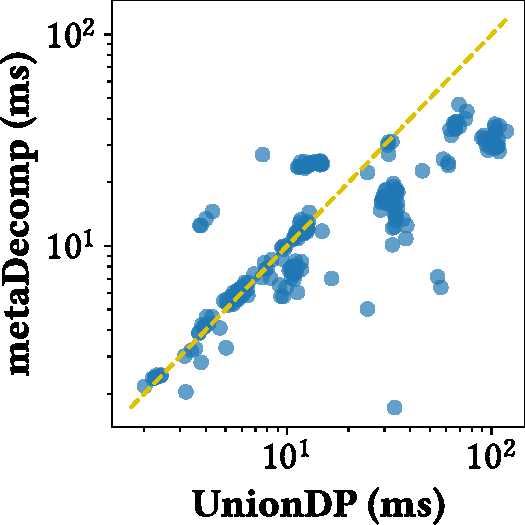
\includegraphics[width=\linewidth]{figs/exp/scatter-individual/scatter-dsb-over-uniondp.pdf}
        \caption{DSB}
        \label{fig:overall-scatter-uniondp-dsb}
    \end{subfigure}
    \hfill
    \begin{subfigure}[b]{0.24\textwidth}
        \centering
        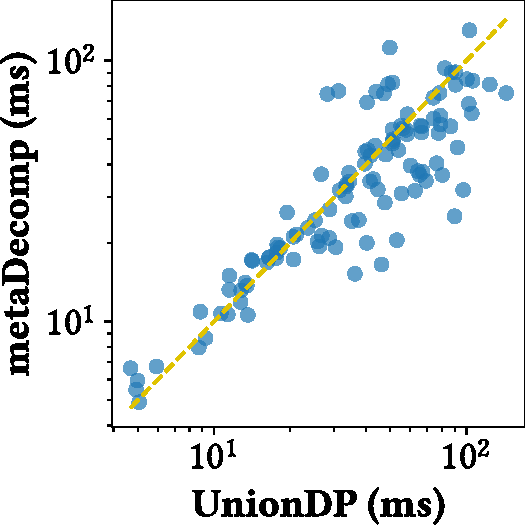
\includegraphics[width=\linewidth]{figs/exp/scatter-individual/scatter-job-original-over-uniondp.pdf}
        \caption{JOB}
        \label{fig:overall-scatter-uniondp-job-original}
    \end{subfigure}
    \hfill
    \begin{subfigure}[b]{0.24\textwidth}
        \centering
        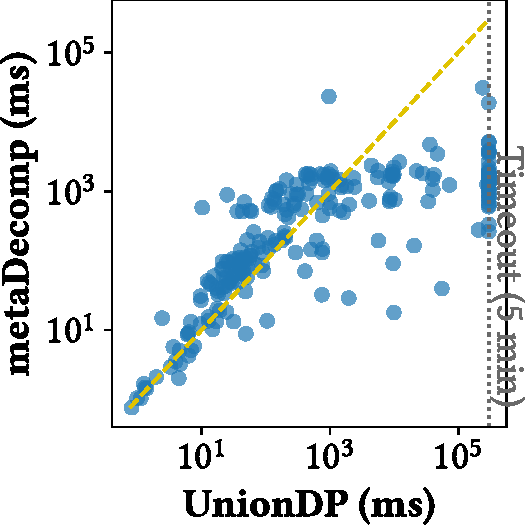
\includegraphics[width=\linewidth]{figs/exp/scatter-individual/scatter-musicbrainz-over-uniondp.pdf}
        \caption{Musicbrainz}
        \label{fig:overall-scatter-uniondp-musicbrainz}
    \end{subfigure}
    \hfill
    \begin{subfigure}[b]{0.24\textwidth}
        \centering
        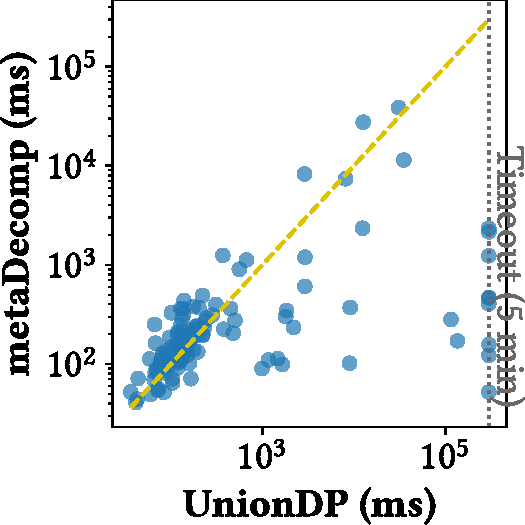
\includegraphics[width=\linewidth]{figs/exp/scatter-individual/scatter-job-large-over-uniondp.pdf}
        \caption{JOBLarge}
        \label{fig:overall-scatter-uniondp-job-large}
    \end{subfigure}
    \vspace{-0.5\baselineskip}
    \caption{Scatter plot of overall evaluation time of using \sys{} versus UnionDP on each benchmark}
    \label{fig:overall-scatter-uniondp-individual}
\end{figure}

\newpage

\subsubsection{\sys{} versus Yannakakis$^+$}
\label{app:total-time-yanplus-individual}
\paragraph{Histograms of speedups}
\cref{fig:overall-speedup-yanplus-individual} shows histograms of the speedups of the overall execution time using \sys{} over using Yannakakis$^+$ for queries in each of the four benchmarks. The major advantage of \sys{} over Yannakakis$^+$ is the elimination of the overhead of full reduction, and this is very clearly reflected in the speedups in the smaller benchmarks DSB and JOB. On the larger benchmarks Musicbrainz and JOBLarge, \sys{} also shows comparable performance, with significant speedups on a few queries in which the full reduction takes a very long time.

\begin{figure}[H]
    \begin{subfigure}[b]{0.49\textwidth}
        \centering
        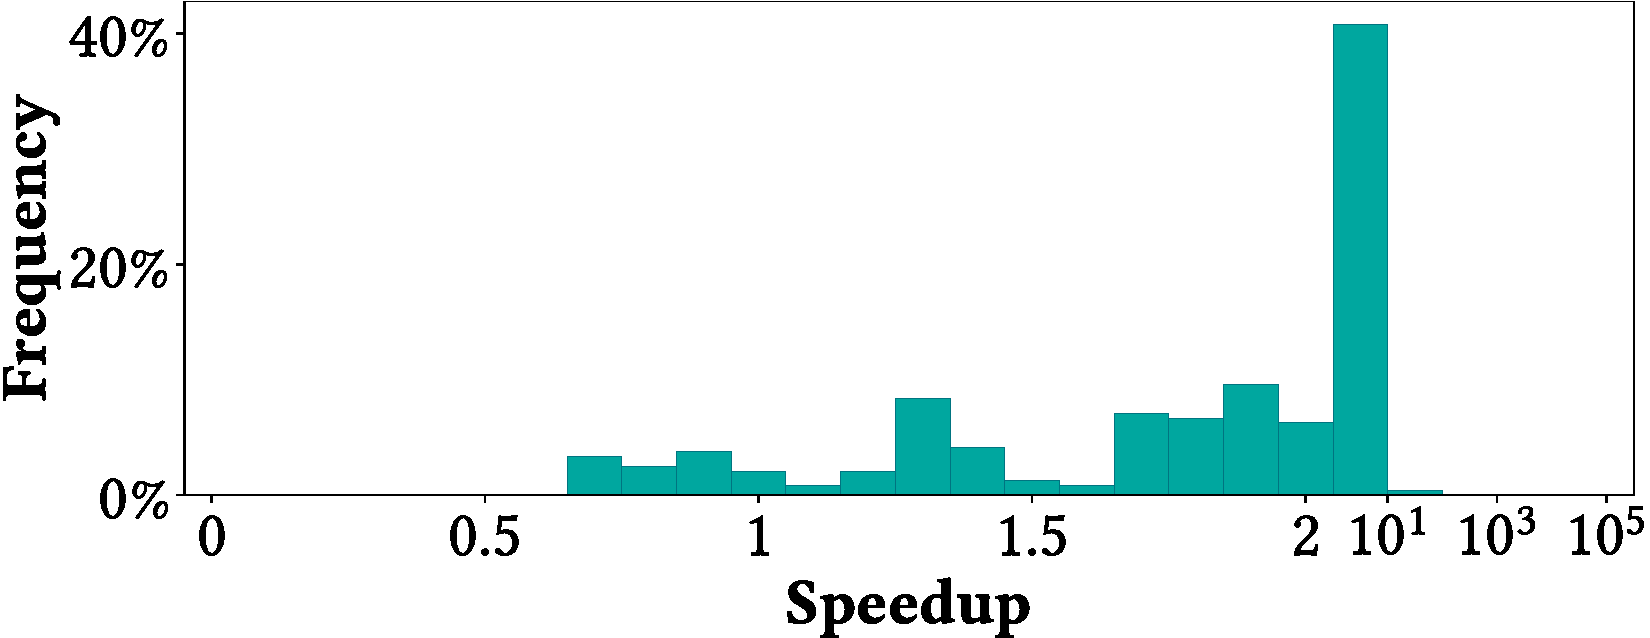
\includegraphics[width=\linewidth]{figs/exp/overall-speedups-individual/overall-speedups-over-yanplus-dsb.pdf}
        \caption{DSB}
        \label{fig:overall-speedup-yanplus-dsb}
    \end{subfigure}
    \hfill
    \begin{subfigure}[b]{0.49\textwidth}
        \centering
        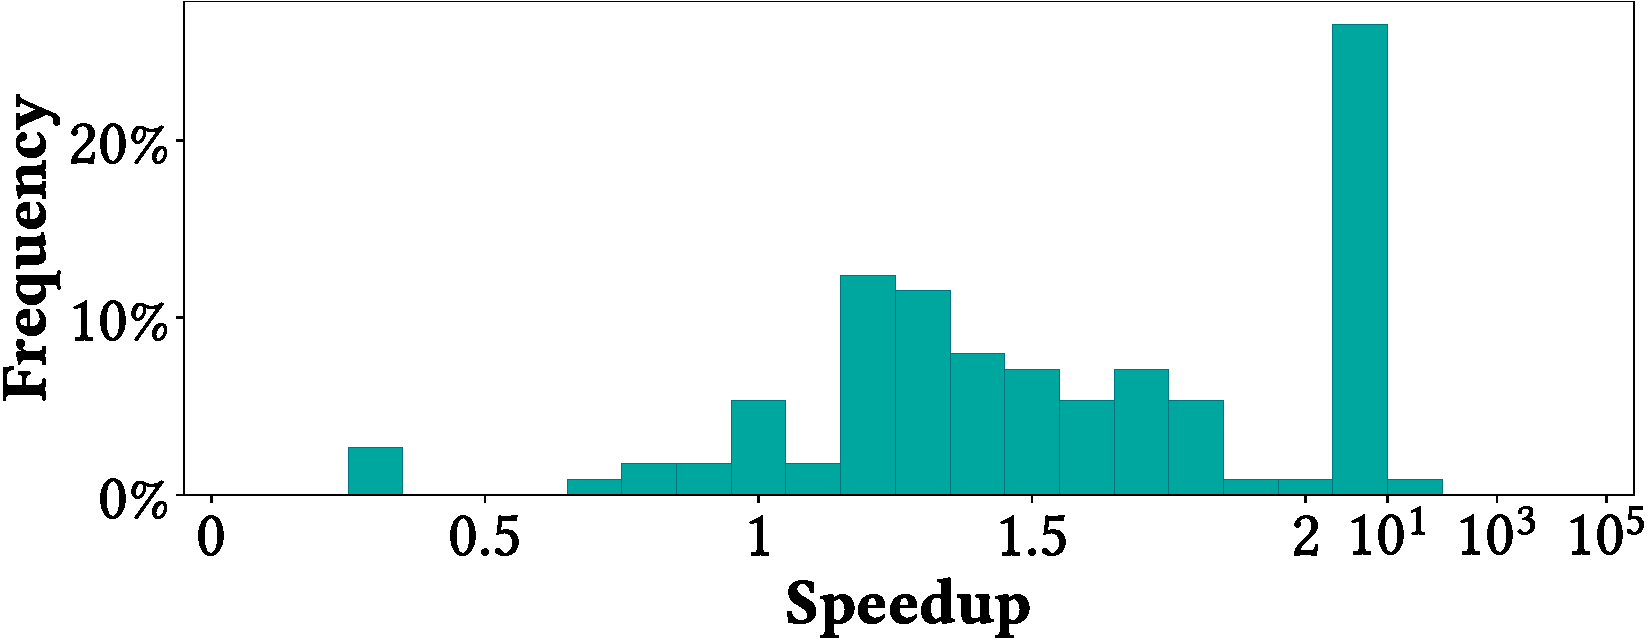
\includegraphics[width=\linewidth]{figs/exp/overall-speedups-individual/overall-speedups-over-yanplus-job-original.pdf}
        \caption{JOB}
        \label{fig:overall-speedup-yanplus-job-original}
    \end{subfigure}

    \vspace{0.5\baselineskip}

    \begin{subfigure}[b]{0.49\textwidth}
        \centering
        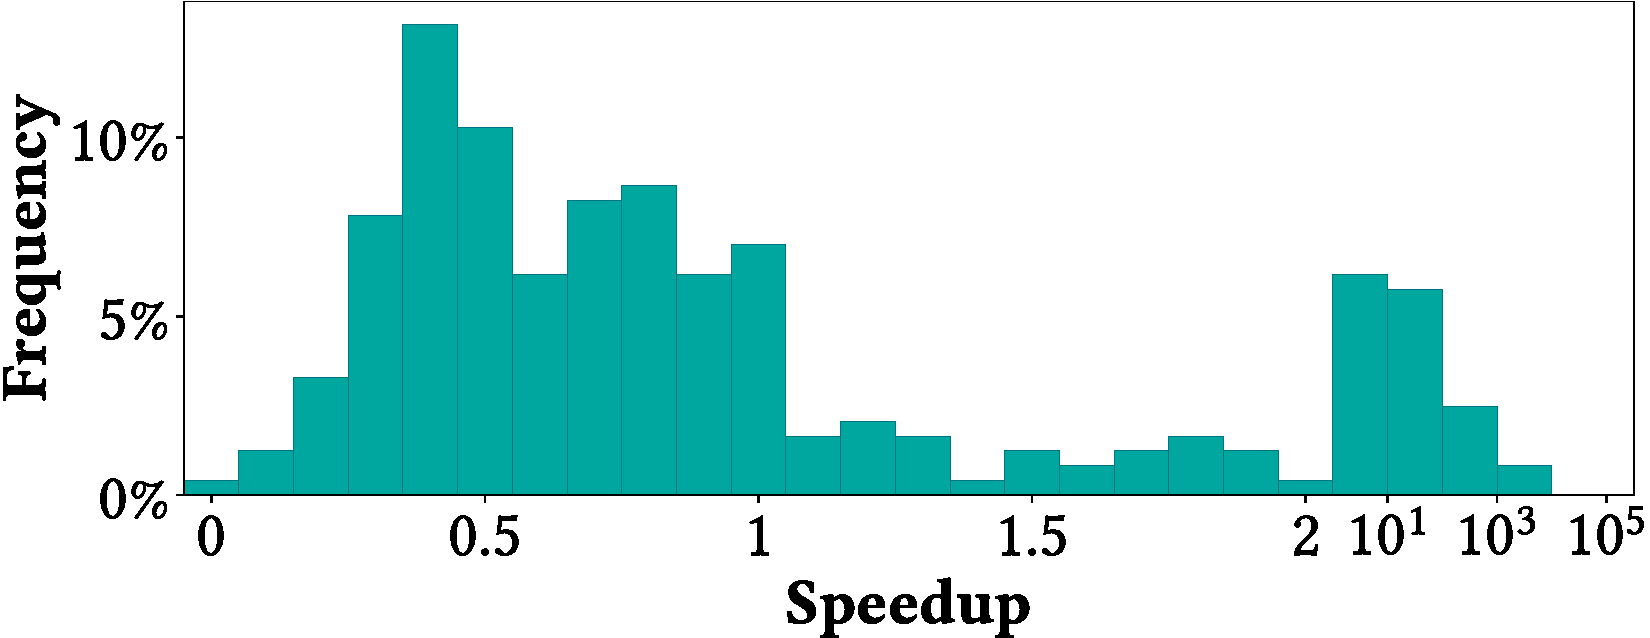
\includegraphics[width=\linewidth]{figs/exp/overall-speedups-individual/overall-speedups-over-yanplus-musicbrainz.pdf}
        \caption{Musicbrainz}
        \label{fig:overall-speedup-yanplus-musicbrainz}
    \end{subfigure}
    \hfill
    \begin{subfigure}[b]{0.49\textwidth}
        \centering
        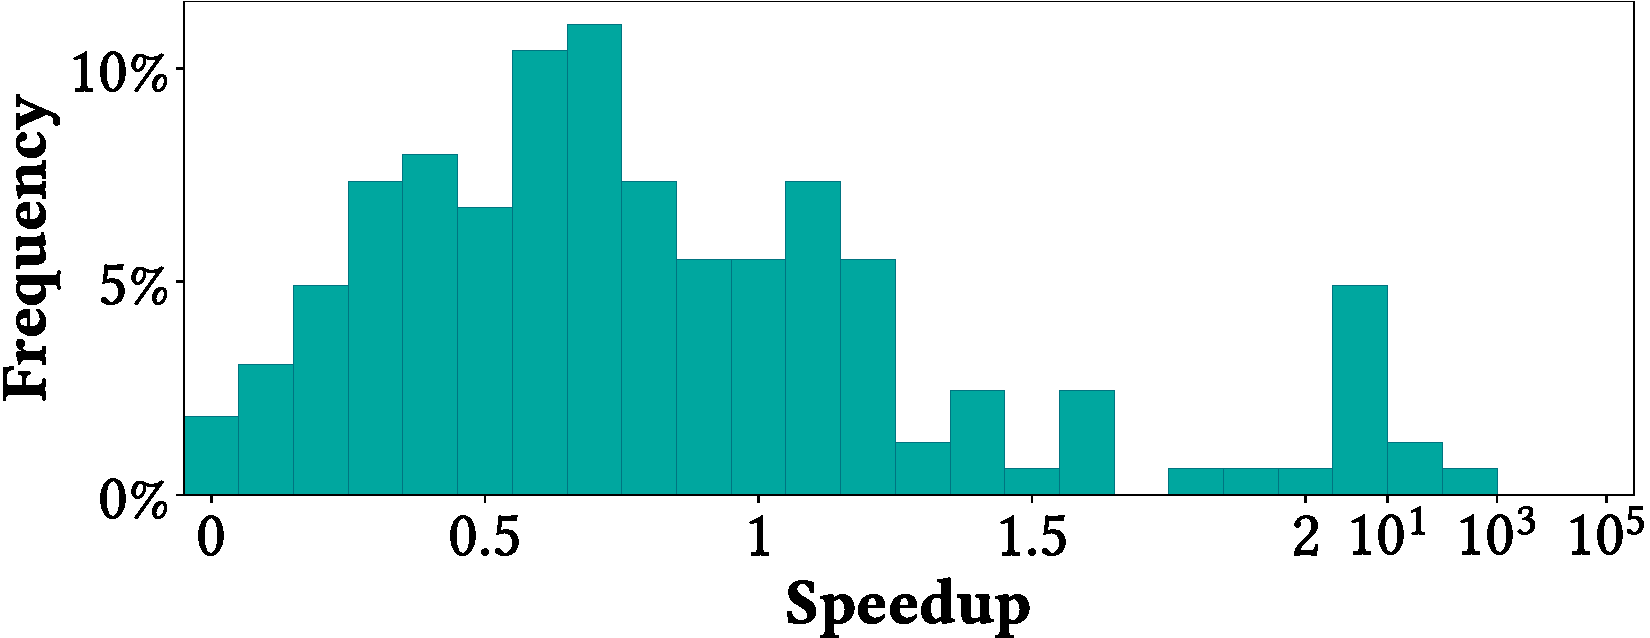
\includegraphics[width=\linewidth]{figs/exp/overall-speedups-individual/overall-speedups-over-yanplus-job-large.pdf}
        \caption{JOBLarge}
        \label{fig:overall-speedup-yanplus-job-large}
    \end{subfigure}
    \vspace{-0.5\baselineskip}
    \caption{Histograms of speedups of overall evaluation time of \sys{} over Yannakakis$^+$ on each benchmark}
    \label{fig:overall-speedup-yanplus-individual}
\end{figure}

\paragraph{Scatter plots} \cref{fig:overall-scatter-yanplus-individual} shows scatter plots of the overall query evaluation time using \sys{} and using Yannakakis$^+$ measured for queries in each of the four benchmarks. Again, the elimination of the overhead of full reduction allows for speedups in many queries in all four benchmarks, and there are significant speedups on a few queries in Musicbrainz and JOBLarge for which the full reduction takes a very long time.

\begin{figure}[H]
    \begin{subfigure}[b]{0.24\textwidth}
        \centering
        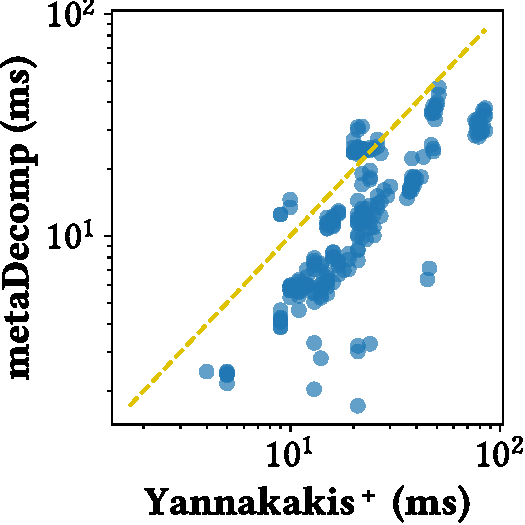
\includegraphics[width=\linewidth]{figs/exp/scatter-individual/scatter-dsb-over-yanplus.pdf}
        \caption{DSB}
        \label{fig:overall-scatter-yanplus-dsb}
    \end{subfigure}
    \hfill
    \begin{subfigure}[b]{0.24\textwidth}
        \centering
        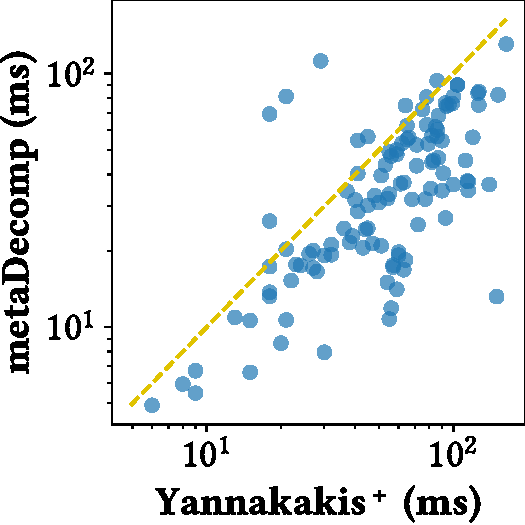
\includegraphics[width=\linewidth]{figs/exp/scatter-individual/scatter-job-original-over-yanplus.pdf}
        \caption{JOB}
        \label{fig:overall-scatter-yanplus-job-original}
    \end{subfigure}
    \hfill
    \begin{subfigure}[b]{0.24\textwidth}
        \centering
        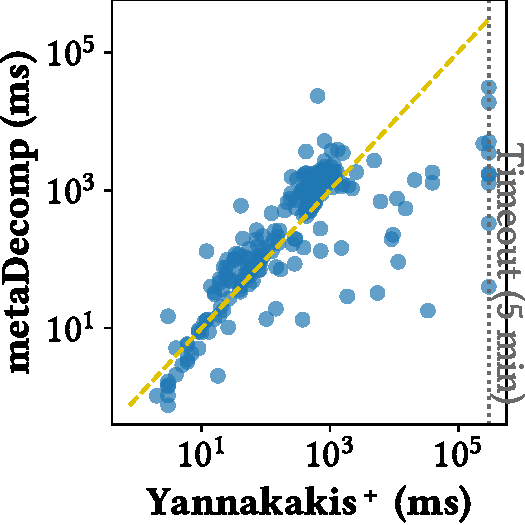
\includegraphics[width=\linewidth]{figs/exp/scatter-individual/scatter-musicbrainz-over-yanplus.pdf}
        \caption{Musicbrainz}
        \label{fig:overall-scatter-yanplus-musicbrainz}
    \end{subfigure}
    \hfill
    \begin{subfigure}[b]{0.24\textwidth}
        \centering
        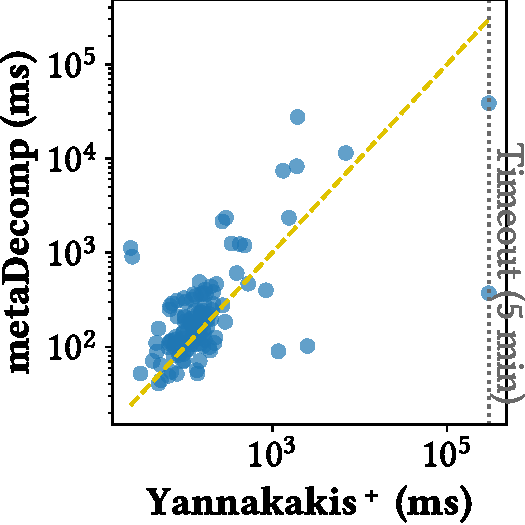
\includegraphics[width=\linewidth]{figs/exp/scatter-individual/scatter-job-large-over-yanplus.pdf}
        \caption{JOBLarge}
        \label{fig:overall-scatter-yanplus-job-large}
    \end{subfigure}
    \vspace{-0.5\baselineskip}
    \caption{Scatter plots of overall evaluation time of using \sys{} versus Yannakakis$^+$ on each benchmark}
    \label{fig:overall-scatter-yanplus-individual}
\end{figure}


\newpage

\subsubsection{\sys{} versus LearnedRewrite}
\label{app:total-time-learned-rewrite-individual}
\paragraph{Histograms of speedups}
\cref{fig:overall-speedup-learned-rewrite-individual} shows histograms of the speedups of the overall execution time using \sys{} over LearnedRewrite for queries in each of the four benchmarks. We can observe a clear overall advantage of \sys{}, due to (1) the large optimization overhead and (2) the limitation of the cost-based optimization and rewrite rules in LearnedRewrite.

\begin{figure}[H]
    \begin{subfigure}[b]{0.49\textwidth}
        \centering
        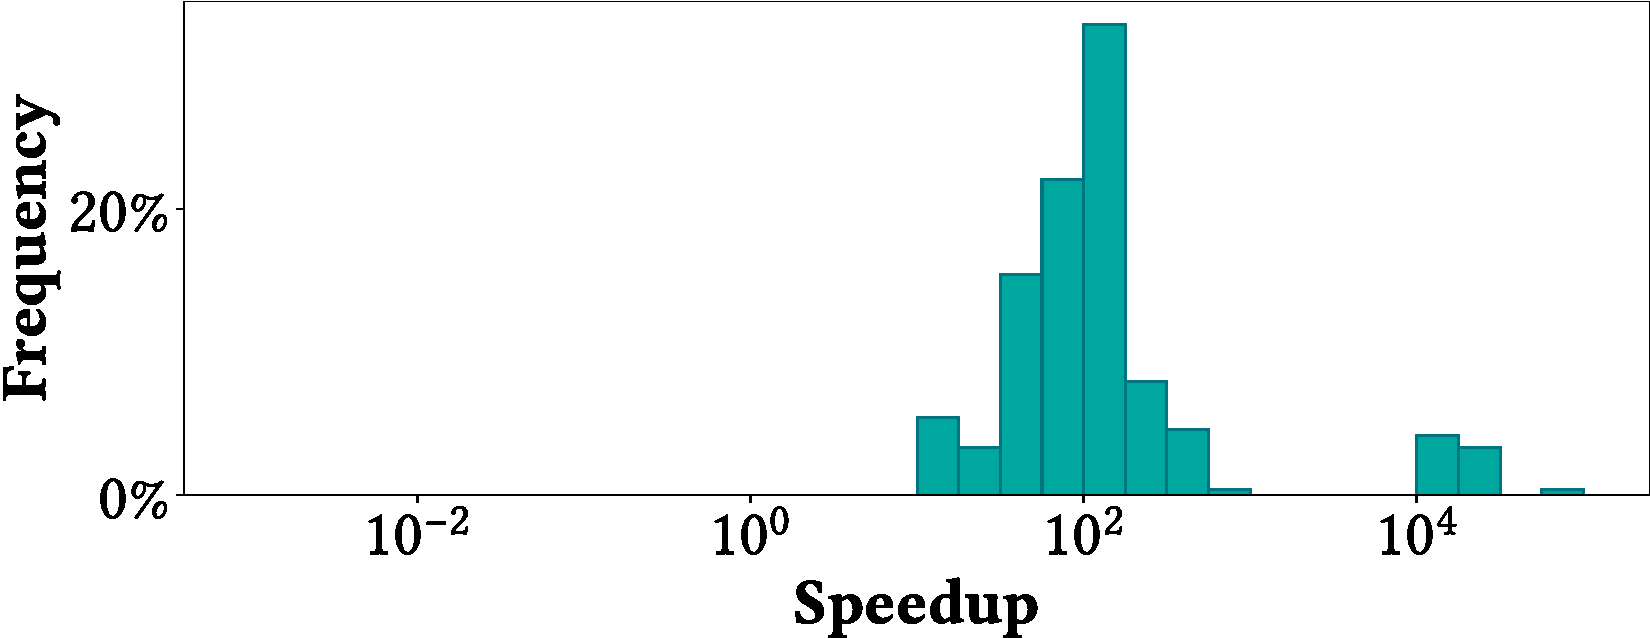
\includegraphics[width=\linewidth]{figs/exp/overall-speedups-individual/overall-speedups-over-learned-rewrite-dsb.pdf}
        \caption{DSB}
        \label{fig:overall-speedup-learned-rewrite-dsb}
    \end{subfigure}
    \hfill
    \begin{subfigure}[b]{0.49\textwidth}
        \centering
        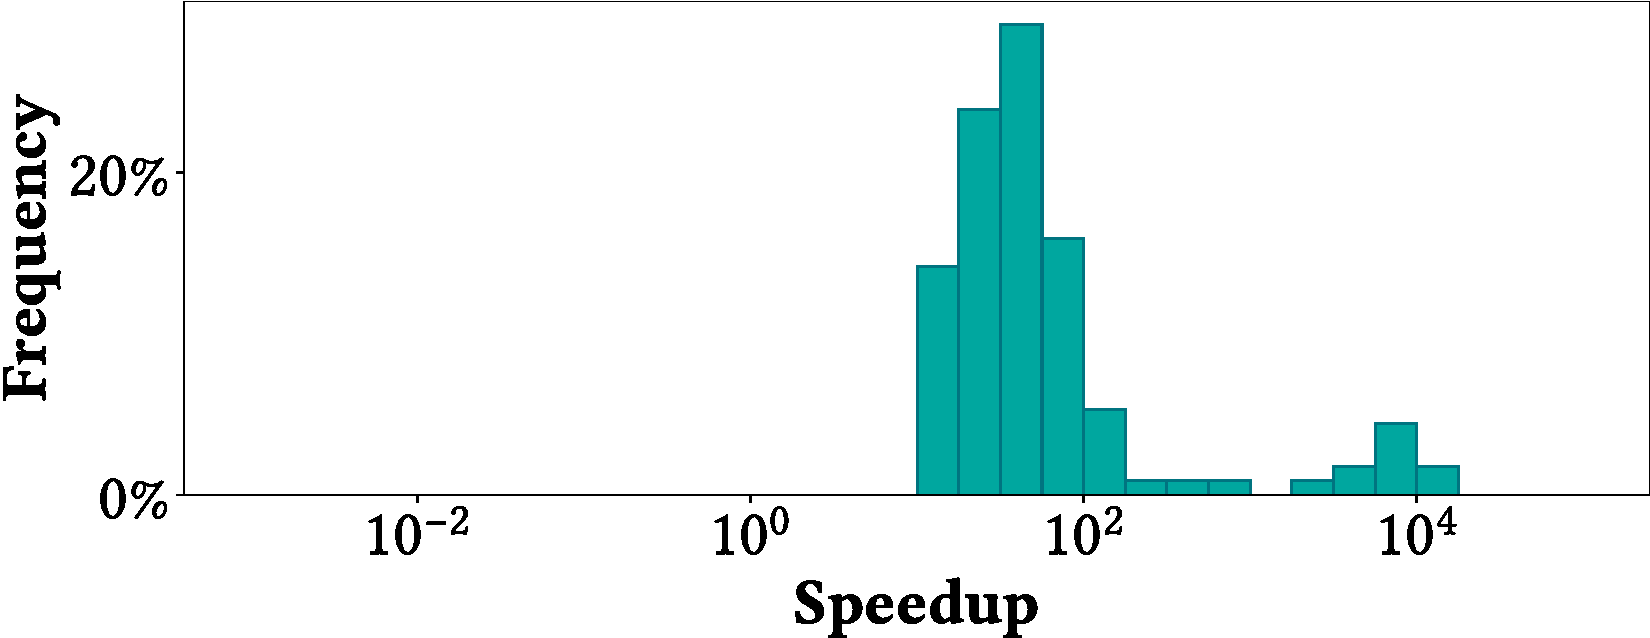
\includegraphics[width=\linewidth]{figs/exp/overall-speedups-individual/overall-speedups-over-learned-rewrite-job-original.pdf}
        \caption{JOB}
        \label{fig:overall-speedup-learned-rewrite-job-original}
    \end{subfigure}

    \vspace{0.5\baselineskip}

    \begin{subfigure}[b]{0.49\textwidth}
        \centering
        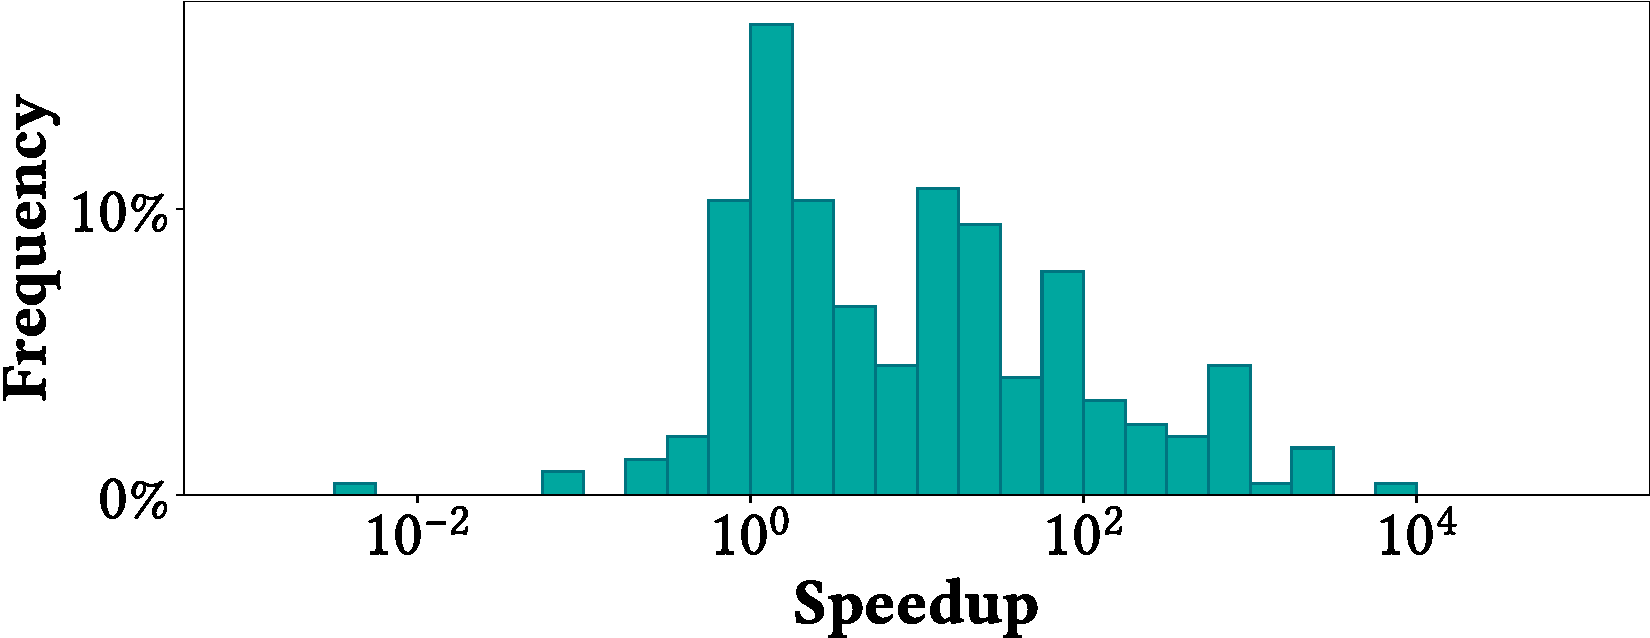
\includegraphics[width=\linewidth]{figs/exp/overall-speedups-individual/overall-speedups-over-learned-rewrite-musicbrainz.pdf}
        \caption{Musicbrainz}
        \label{fig:overall-speedup-learned-rewrite-musicbrainz}
    \end{subfigure}
    \hfill
    \begin{subfigure}[b]{0.49\textwidth}
        \centering
        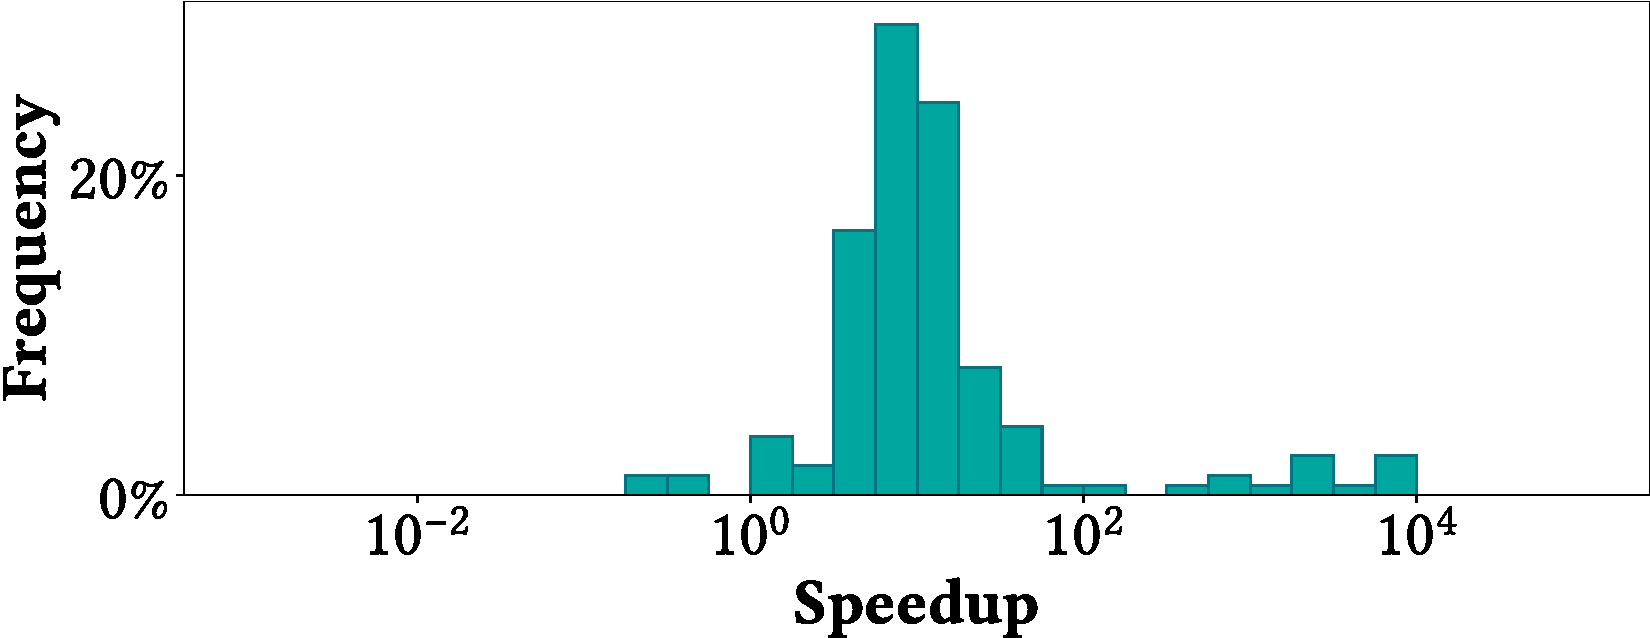
\includegraphics[width=\linewidth]{figs/exp/overall-speedups-individual/overall-speedups-over-learned-rewrite-job-large.pdf}
        \caption{JOBLarge}
        \label{fig:overall-speedup-learned-rewrite-job-large}
    \end{subfigure}
    \vspace{-0.5\baselineskip}
    \caption{Histograms of speedups of overall evaluation time of \sys{} over LearnedRewrite on each benchmark}
    \label{fig:overall-speedup-learned-rewrite-individual}
\end{figure}


\paragraph{Scatter plots} \cref{fig:overall-scatter-learned-rewrite-individual} shows scatter plots of the overall query evaluation time using \sys{} and using Learned Rewrite, measured for queries in each of the four benchmarks. Again, we observe a clear overall advantage of \sys{} over Learned Rewrite in all four benchmarks. In particular, it takes Learned Rewrite an overhead of at least 1 second to optimize each query. For many small queries, this is already more than the overall evaluation time for \sys{} as well as other traditional query optimization approaches.

\begin{figure}[H]
    \begin{subfigure}[b]{0.24\textwidth}
        \centering
        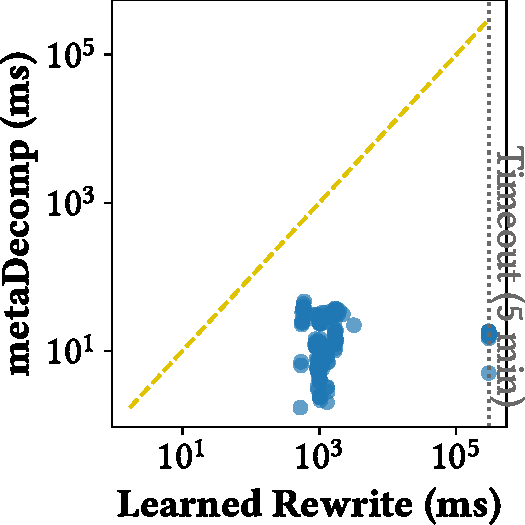
\includegraphics[width=\linewidth]{figs/exp/scatter-individual/scatter-dsb-over-learned-rewrite.pdf}
        \caption{DSB}
        \label{fig:overall-scatter-learned-rewrite-dsb}
    \end{subfigure}
    \hfill
    \begin{subfigure}[b]{0.24\textwidth}
        \centering
        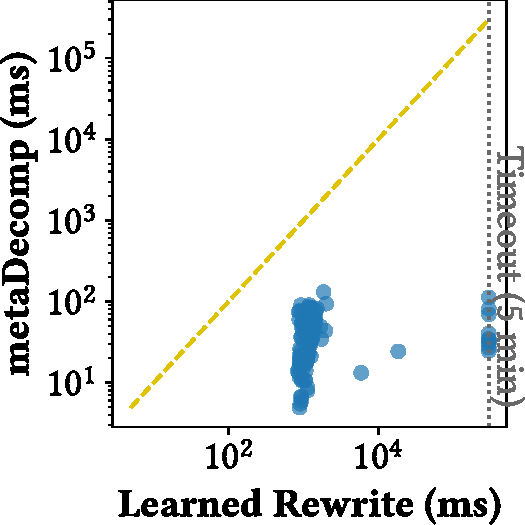
\includegraphics[width=\linewidth]{figs/exp/scatter-individual/scatter-job-original-over-learned-rewrite.pdf}
        \caption{JOB}
        \label{fig:overall-scatter-learned-rewrite-job-original}
    \end{subfigure}
    \hfill
    \begin{subfigure}[b]{0.24\textwidth}
        \centering
        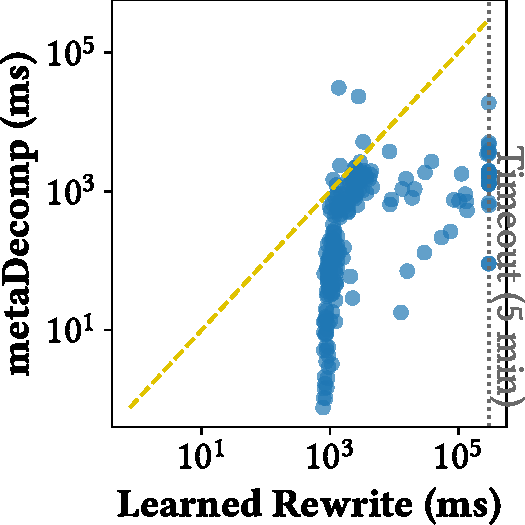
\includegraphics[width=\linewidth]{figs/exp/scatter-individual/scatter-musicbrainz-over-learned-rewrite.pdf}
        \caption{Musicbrainz}
        \label{fig:overall-scatter-learned-rewrite-musicbrainz}
    \end{subfigure}
    \hfill
    \begin{subfigure}[b]{0.24\textwidth}
        \centering
        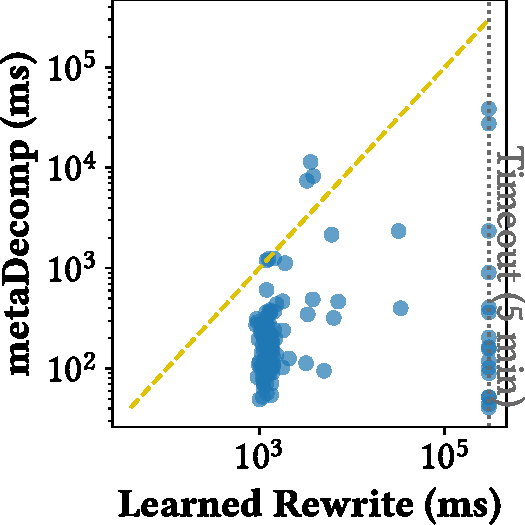
\includegraphics[width=\linewidth]{figs/exp/scatter-individual/scatter-job-large-over-learned-rewrite.pdf}
        \caption{JOBLarge}
        \label{fig:overall-scatter-learned-rewrite-job-large}
    \end{subfigure}
    \vspace{-0.5\baselineskip}
    \caption{Scatter plots of overall evaluation time using \sys{} versus LearnedRewrite on each benchmark}
    \label{fig:overall-scatter-learned-rewrite-individual}
\end{figure}


\newpage

\subsubsection{\sys{} versus LLM-R$^2$}
\label{app:total-time-llm-r2-individual}
\paragraph{Histograms of speedups}
\cref{fig:overall-speedup-llm-r2-individual} shows histograms of the speedups of the overall query execution time using \sys{} over using LLM-R$^2$ for queries in each of the four benchmarks. Similar to the case for Learned Rewrite, we can observe a clear overall advantage of \sys{} over LLM-R$^2$, due to (1) the large optimization overhead and (2) the limitation of the cost-based optimization and rewrite rules of LLM-R$^2$.

\begin{figure}[H]
    \begin{subfigure}[b]{0.49\textwidth}
        \centering
        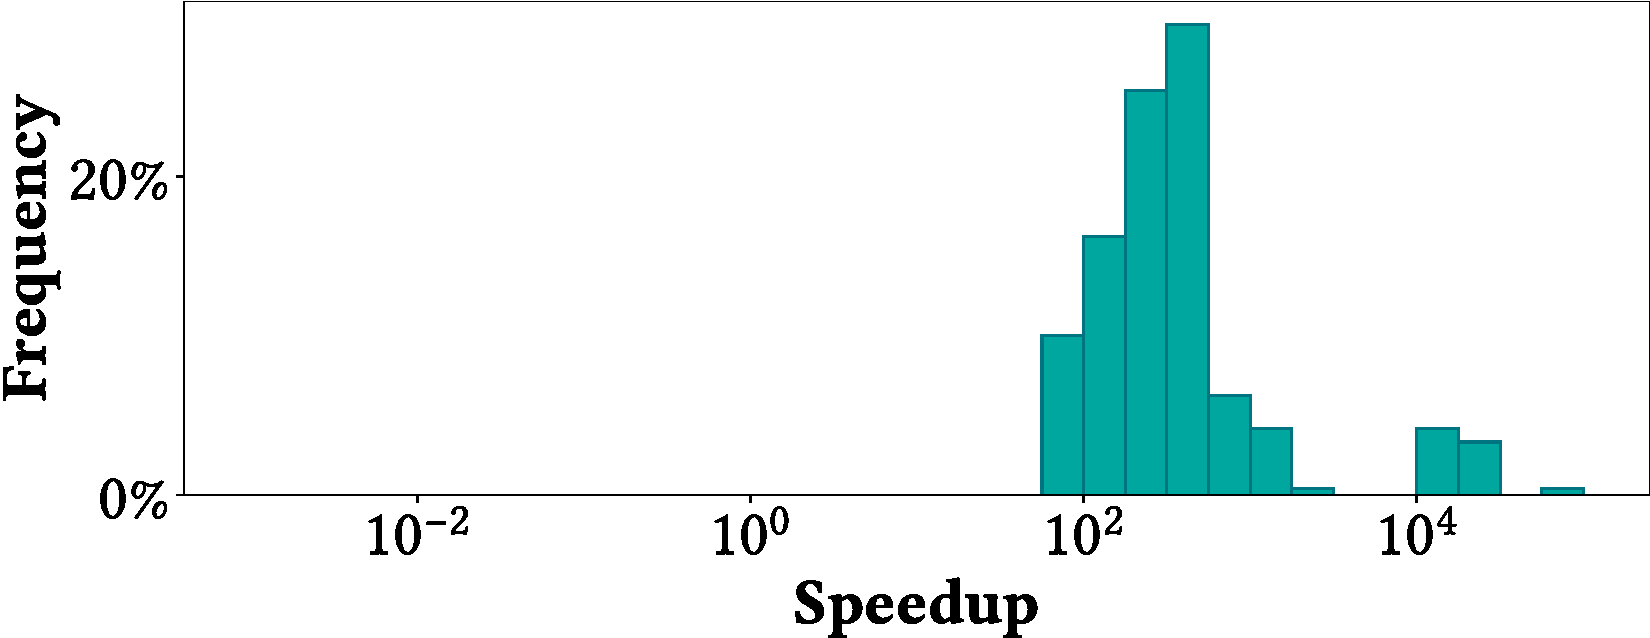
\includegraphics[width=\linewidth]{figs/exp/overall-speedups-individual/overall-speedups-over-llm-r2-dsb.pdf}
        \caption{DSB}
        \label{fig:overall-speedup-llm-r2-dsb}
    \end{subfigure}
    \hfill
    \begin{subfigure}[b]{0.49\textwidth}
        \centering
        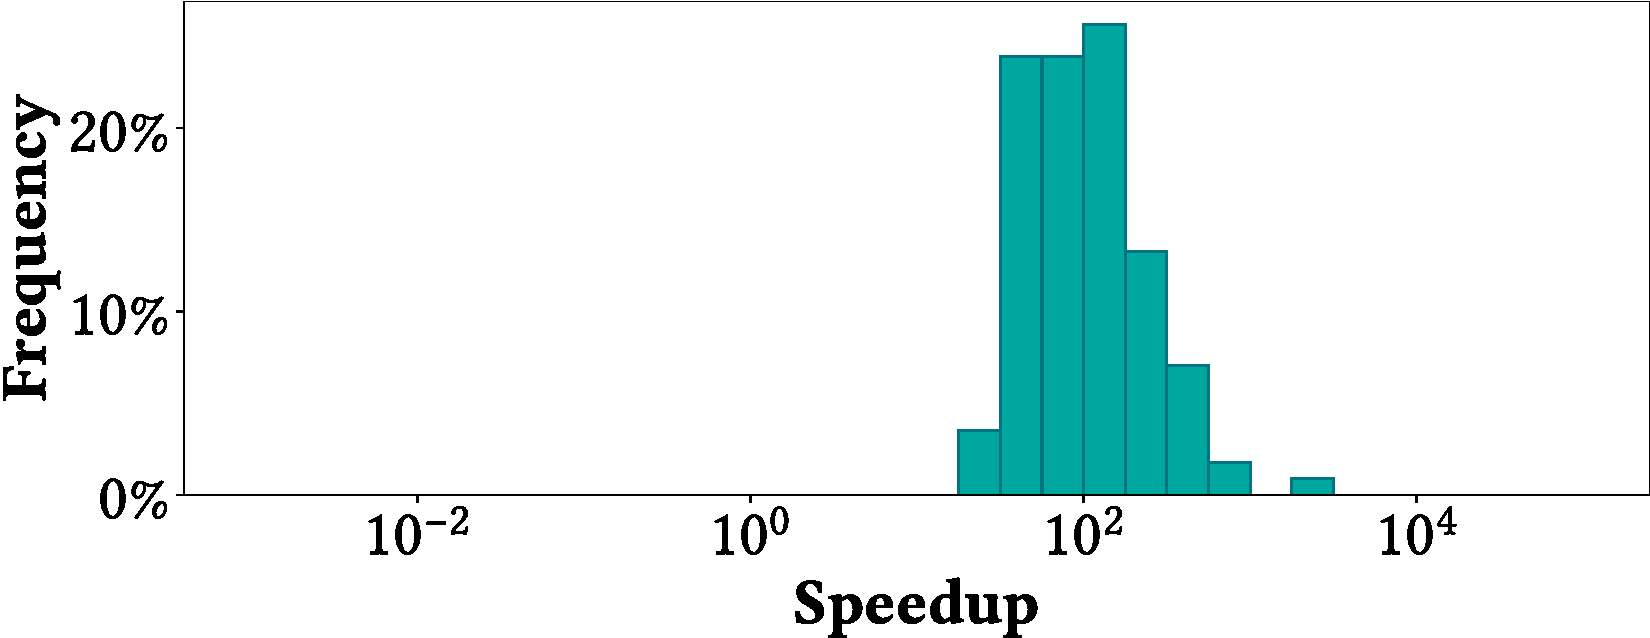
\includegraphics[width=\linewidth]{figs/exp/overall-speedups-individual/overall-speedups-over-llm-r2-job-original.pdf}
        \caption{JOB}
        \label{fig:overall-speedup-llm-r2-job-original}
    \end{subfigure}

    \vspace{0.25\baselineskip}

    \begin{subfigure}[b]{0.49\textwidth}
        \centering
        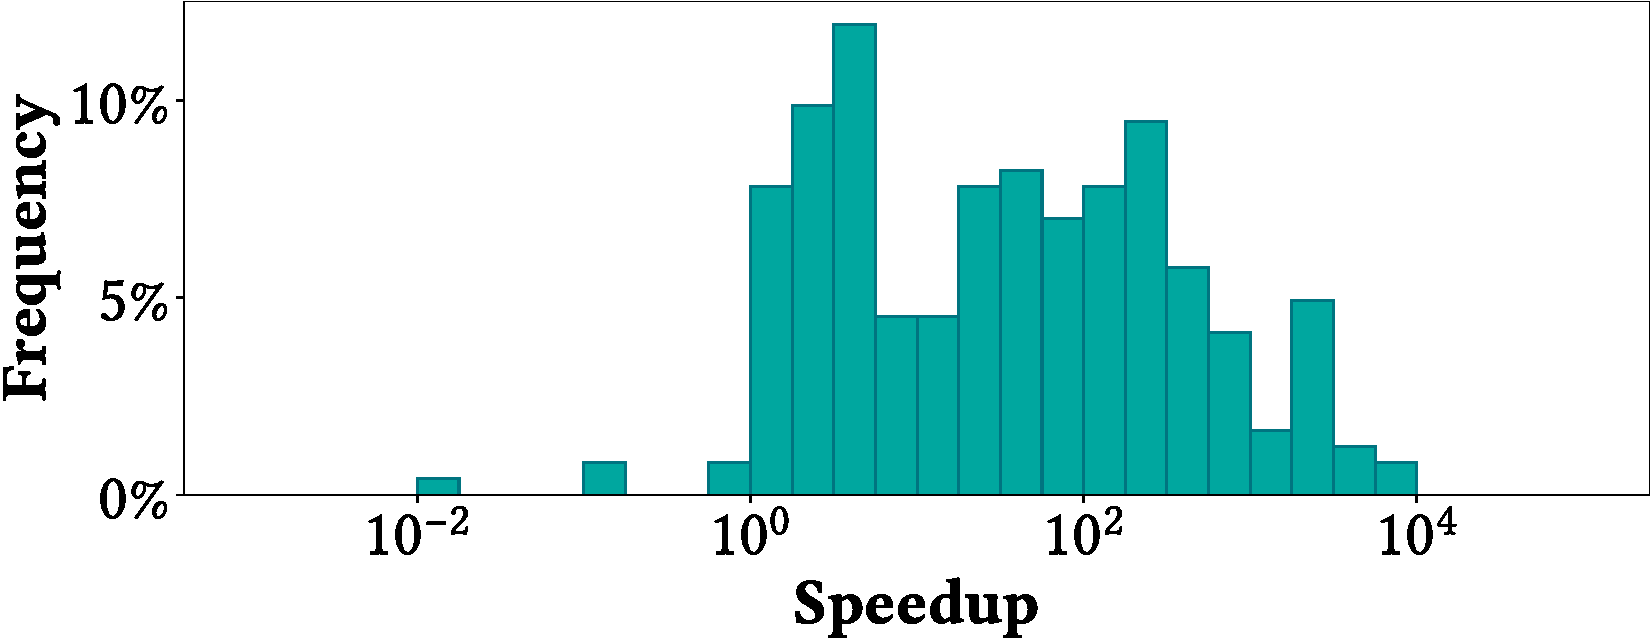
\includegraphics[width=\linewidth]{figs/exp/overall-speedups-individual/overall-speedups-over-llm-r2-musicbrainz.pdf}
        \caption{Musicbrainz}
        \label{fig:overall-speedup-llm-r2-musicbrainz}
    \end{subfigure}
    \hfill
    \begin{subfigure}[b]{0.49\textwidth}
        \centering
        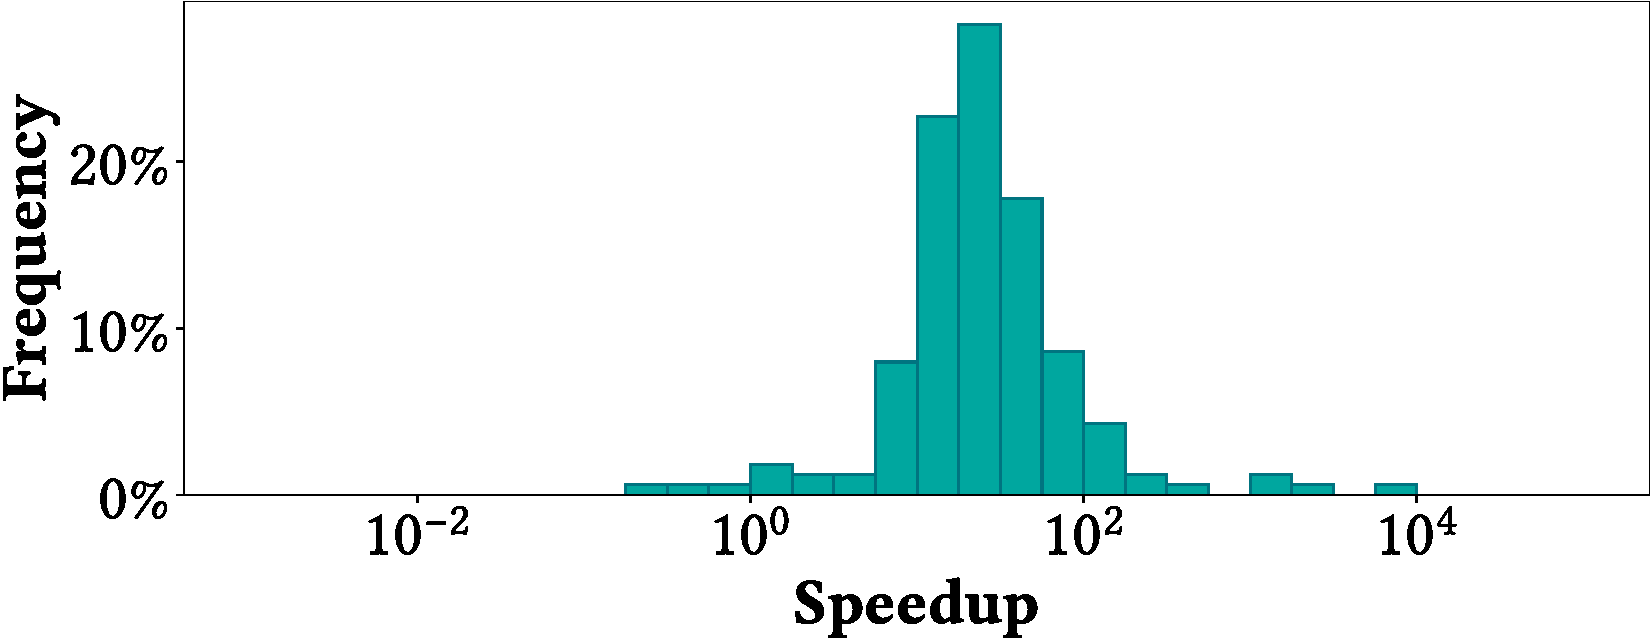
\includegraphics[width=\linewidth]{figs/exp/overall-speedups-individual/overall-speedups-over-llm-r2-job-large.pdf}
        \caption{JOBLarge}
        \label{fig:overall-speedup-llm-r2-job-large}
    \end{subfigure}
    \vspace{-0.5\baselineskip}
    \caption{Histograms of speedups of overall evaluation time of \sys{} over LLM-R$^2$ on each benchmark}
    \label{fig:overall-speedup-llm-r2-individual}
\end{figure}


\paragraph{Scatter plots} \cref{fig:overall-scatter-llm-r2-individual} shows scatter plots of the overall query evaluation time using \sys{} and using LLM-R$^2$, measured for queries in each of the four benchmarks. Again, we observe a clear overall advantage of \sys{} over LLM-R$^2$ in all four benchmarks. Similar to the case with Learned Rewrite, it takes LLM-R$^2$ an even higher overhead of at least 3 seconds to optimize each query. For many small queries, this is already more than the overall evaluation time for \sys{} as well as other traditional query optimization approaches.

\begin{figure}[H]
    \begin{subfigure}[b]{0.24\textwidth}
        \centering
        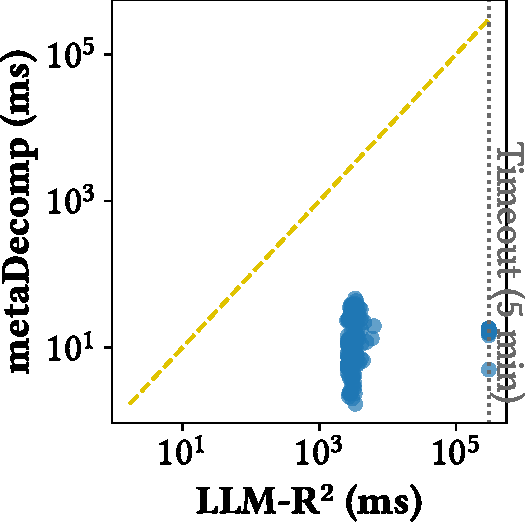
\includegraphics[width=\linewidth]{figs/exp/scatter-individual/scatter-dsb-over-llm-r2.pdf}
        \caption{DSB}
        \label{fig:overall-scatter-llm-r2-dsb}
    \end{subfigure}
    \hfill
    \begin{subfigure}[b]{0.24\textwidth}
        \centering
        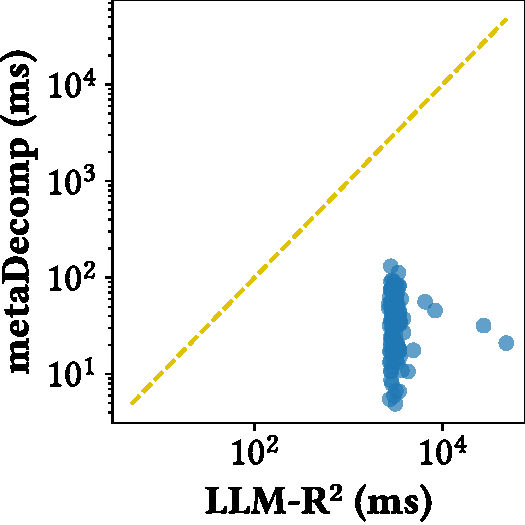
\includegraphics[width=\linewidth]{figs/exp/scatter-individual/scatter-job-original-over-llm-r2.pdf}
        \caption{JOB}
        \label{fig:overall-scatter-llm-r2-job-original}
    \end{subfigure}
    \hfill
    \begin{subfigure}[b]{0.24\textwidth}
        \centering
        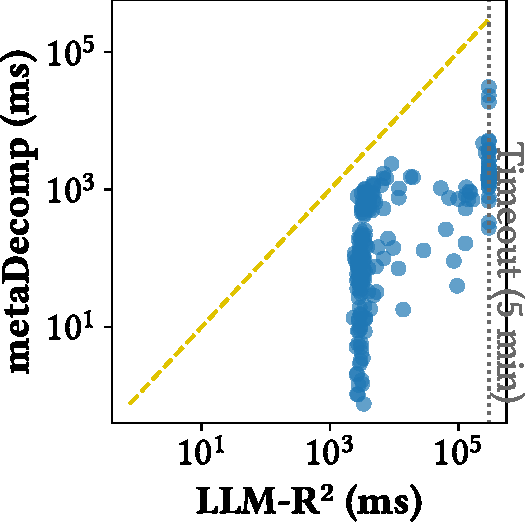
\includegraphics[width=\linewidth]{figs/exp/scatter-individual/scatter-musicbrainz-over-llm-r2.pdf}
        \caption{Musicbrainz}
        \label{fig:overall-scatter-llm-r2-musicbrainz}
    \end{subfigure}
    \hfill
    \begin{subfigure}[b]{0.24\textwidth}
        \centering
        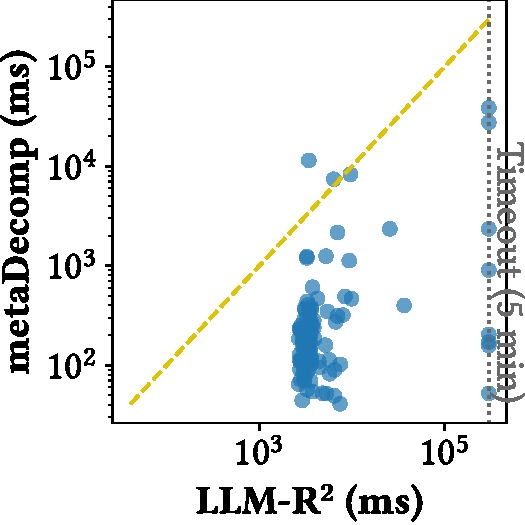
\includegraphics[width=\linewidth]{figs/exp/scatter-individual/scatter-job-large-over-llm-r2.pdf}
        \caption{JOBLarge}
        \label{fig:overall-scatter-llm-r2-job-large}
    \end{subfigure}
    \vspace{-0.5\baselineskip}
    \caption{Scatter plot of overall evaluation time of using \sys{} versus LLM-R$^2$ on each benchmark}
    \label{fig:overall-scatter-llm-r2-individual}
\end{figure}


